\clearpage
\chapter{PV Cell Orientation Angles Optimization for a Base Station Equipped with Several PV Cells\label{Chapter_1}}

\section{Literature Review: Orientation Angle Optimization}
Many papers in the literature map for a given PV cell its performance in a wide geographical area. The average yearly or daily energy output of the PV cell is used as the performance metric. For each geographical location in the investigated area, the latitude, the longitude, the altitude, the ambient temperature, the wind speed, the solar spectrum, and site-specific weather conditions are often used to determine the performance of the PV cell. Nonetheless, these papers do not optimize any of the parameters of the PV cell, such as the orientation angle, instead they derive a guideline for the best deployment area for the given PV cell type. For example, \cite{south_africa}, \cite{HuldThomas2010Mtpo} and \cite{ThomasHuld2015EPMP} derive comprehensive guides for PV cell deployment areas in South Africa, Europe, and Eurasia, respectively.  
In addition, geographic information systems (GISs) provide such guides for various geographical areas online, such as for the USA \cite{usa}, for Europe \cite{PVGIS}, and worldwide \cite{worldwide,worldwide2}. 



Most papers investigating differently oriented PV cells, such as \cite{ORDONEZ20102122}, have not actually optimized the PV cell angles but considered some deployment constraints, e.g., that the PV cells are mounted on residential rooftops, which predefine the PV cell angles. 

Other papers, such as \cite{VALLADARESRENDON2017458}, optimize the orientation of objects to increase or decrease the sun irradiance on the object. These objects do not have to be PV cells. For example, \cite{VALLADARESRENDON2017458} determines the optimal orientation of a building (no PV cells are deployed) so that less sun irradiance can enter the building through the windows. In climates with abundant sun irradiance, orientating the buildings so that less irradiance can enter the buildings through the windows reduces the need for cooling the buildings with air conditioning.


PV cell angle optimization for maximizing the total energy output of the PV cells has been done for Singapore in \cite{irradianceModels}, however, without considering the potential mismatch between the energy generation profile of the PV cells and the energy consumption profile of the appliance. This may result in service outage if the PV cells are the only energy source or additional expenditures if the energy deficit has to be compensated by using alternative energy sources. Different from \cite{irradianceModels}, the optimal PV cell orientation angles are derived in this thesis to match a given energy consumption profile rather than maximizing the total energy output of the PV cells. 

In \cite{Kemery2012OptimalPO}, the PV cell angle optimization considered the energy demand of the Ontario province of Canada, where the authors investigated orientation angles from $15^\mathrm{o}$ east of due south to $15^\mathrm{o}$ west of due south, i.e., $\theta\in[-15^{\mathrm{o}},15^{\mathrm{o}}]$. But propagation losses along the power lines among the widely-distributed PV cell installations were not included, which are significant factors when operating on a provincial scale \cite{8491374,my_con3}. Different from \cite{Kemery2012OptimalPO}, the optimal PV cell orientation angles are derived in the range from east ($\theta=-90^\mathrm{o}$) to west ($\theta=90^\mathrm{o}$) in this thesis.

The authors of \cite{CHATTOPADHYAY2017176} investigated five orientation angle settings (east, southeast, south, southwest, and west) and concluded that in some scenarios a mix of east-oriented and west-oriented PV cells and in other scenarios south-oriented PV cells reduce the needs for storage and backup from dispatchable energy sources in a fully renewable European power system. Because they adjusted the installed capacity of the PV cells for each angle configuration, such that the average power production of each PV cell remains the same, it is difficult to fairly judge if the reduced needs for storage and backup are a good trade-off for the increased installed capacity of PV cells. Different from \cite{CHATTOPADHYAY2017176}, the installed capacity of the PV cells is kept unchanged in this thesis. Hence, it is possible to fairly present the improvements caused by different PV cell orientation angles in this thesis.


Optimizing the PV cell inclination angle to power an isolated island was studied in \cite{7315106}, where the PV cell inclination angle was optimized on a yearly timescale. Because the PV cell inclination angle was optimized, the energy can be shifted on a yearly timescale, i.e., from a surplus season (e.g. summer) to a deficit season (e.g. winter), but the energy cannot be shifted on a daily timescale, i.e., from a surplus time (e.g. noon) to a deficit time (e.g. morning or afternoon) with the proposed method in \cite{7315106}.  



In my papers \cite{my,my2,my4}, I have been optimizing the PV cell orientation angle of one PV cell deployed at the BS to match the energy generation of this single PV cell with the energy consumption of a BS. Optimizing the PV cell orientation angle of several PV cells deployed at the BS to match the energy generation of the PV cells with the energy consumption of a BS has been studied in my paper \cite{sub}. Hence, my paper \cite{sub} is an extension to my previous papers \cite{my,my2,my4}. Chapter \ref{Chapter_1} of this thesis is based on \cite{sub}. In contrast to \cite{my,my2,my4}, \cite{sub} can investigate how the number of PV cells and the composition of differently oriented PV cells improve the match between the energy generation profile of the PV cells and the energy consumption profile of the BS.

\section{Contributions of Chapter \ref{Chapter_1}}
The contributions of Chapter \ref{Chapter_1} are summarized as follows:

\begin{itemize}
\item Developing an algorithm to jointly optimize the orientation angles of several PV cells powering one BS. The algorithm achieves the best possible match between the energy generation profiles of the PV cells and the energy consumption profile of the BS. The proposed optimization algorithm only needs to be run a single time offline and the obtained optimal angles can be used for all solar-powered BSs with similar geographic locations and energy consumption profiles.
\item Deriving analytically the irradiance values on any randomly inclined and oriented PV cell. A horizontally-mounted PV cell is used as a baseline and its irradiance values have to be given to derive the irradiance values on any randomly inclined and oriented PV cell at the same location.
\item Identifying and discussing analytically to what extent the orientation angle $\theta$ shifts the energy generation profile away from noon if the PV cells are not south-oriented ($\theta \neq 0^\mathrm{o}$).  
\item Evaluating the effectiveness of the proposed orientation angle optimization on three different types of BS energy consumption profiles: constant traffic load profiles, business-area traffic load profiles, and residential-area traffic load profiles. The energy drawn from the main grid by the BS per day is used as the performance metric.
\item Giving recommendations on how many differently oriented PV cells should be deployed for a given energy consumption profile. To the best of my knowledge, this has never been investigated in the literature before.
\end{itemize}



\section{System Model 1 - Several PV Cells Powering One BS\label{system_1}}
Figure \ref{ene} depicts the system model 1 considered in Chapter \ref{Chapter_1}. The energy generation part consists of $N$ identical PV cells, denoted by PV cell 1, PV cell 2, ..., and PV cell $N$, $N \in \mathbb{N}$. The energy consumption part consists of a BS. The total surface area of all $N$ PV cells is $A$. Each PV cell has a surface area of $\frac{A}{N}$. The day is divided into $T$ time steps, $T\in\mathbb{N}$. The index of a time step is denoted by $t$, $t \in \{1,...,T\}$.
The BS uses the energy generated by the $N$ PV cells, denoted by $G(t)$, to support its energy consumption $C(t)$ at every time step $t$. 
If there is an energy deficit, i.e., $C(t)-G(t)>0$, the BS draws the remaining energy from the main grid at time step $t$. If there is an energy surplus, i.e., $C(t)-G(t)<0$, the surplus energy is wasted at time step $t$ or fed to the grid\footnote{There are no feed-in tariffs considered in this thesis because I want to incentify that the generated energy is used locally. Large amounts of intermittent generated energy which is fed into the grid often causes unbalancing issues, and voltage drops in the grid or in the worst-case scenario a black out. Matching the energy generation profile with the energy consumption profile on-site at a BS reduces therefore the stress on the power grid. This assumption is justified because most power grids nowadays are still designed for one-directional energy flow from a few large-scale centralized energy generators, such as coal power plants or nuclear power plants, to many small-scale energy consumers, such as domestic households or BSs. Current power grid infrastructure is often not assigned to accommodate huge amounts of energy flow in opposite direction and to redistribute such intermittent generated energy sufficiently without causing grid instability or jeopardizing the reliability of the power grid. Even if surplus energy can be sold to the grid, the system model 1 aims to match the energy generation profile with the energy consumption profile on-site at a BS, which is more cost-effective for the BS/ PV cells owner than wasting the surplus energy or selling the surplus energy to the grid for redistribution. Grid  operators always sell energy at a higher price than they buy it.}


The optimization object in the system model 1 is to minimize the amount of energy that has to be drawn from the main grid by the BS on a daily time scale. The energy drawn from the main grid can only be altered by choosing different orientation angles $\theta_1$, ..., and $\theta_N$ for PV cell 1, ..., and PV cell $N$, respectively. All the other parameters of the system, including the inclination angles of all $N$ PV cells, are fixed. In this thesis, the system is located in Greenwich (London, UK) as example, i.e., the Latitude $lat$, and the Longitude $lon$ are fixed to $51.4767^{\mathrm{o}}$ North, and $0.0003^{\mathrm{o}}$ West, respectively, but the analysis can be applied to other locations as well. Hence, all formulas in this thesis are given for a location in the northern hemisphere.


\begin{figure}[H]
\centering
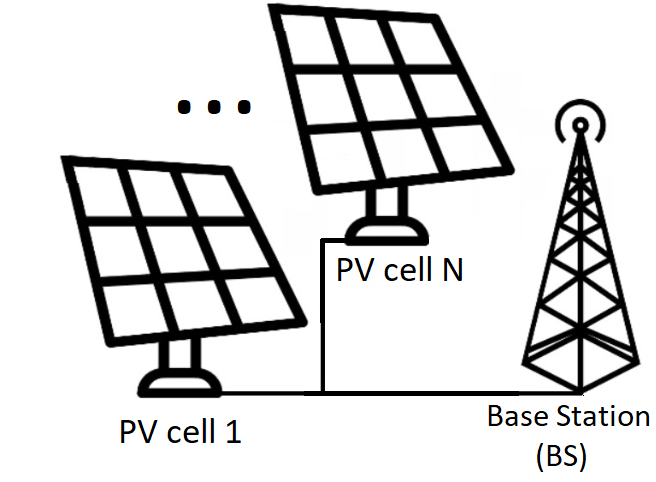
\includegraphics[width=0.6\columnwidth]{pictures/SystemSetup}
\caption{Illustration of system model 1\label{ene}}
\end{figure}

\subsection{Energy Generation of a PV Cell\label{gen}}

A horizontally-mounted PV cell in Greenwich (London, UK) is used as the baseline. From this baseline, a method will be developed to calculate the energy generated by a PV cell at the same location but installed with any orientation angle $\theta \in [-90^{\mathrm{o}},90^{\mathrm{o}}]$ and any inclination angle $\gamma\in[0,90^\mathrm{o}]$. The time is modeled in discrete time steps denoted by the time step index $t$, $t \in \{1,...,T\}$, hence all variables dependent on $t$ are discrete. The global horizontal irradiance $GHI_t$, the diffuse horizontal irradiance $DHI_t$, and the direct normal irradiance $DNI_t$ for a horizontally-mounted PV cell in Greenwich (London, UK) are obtained from the PVGIS database (cf. Figure \ref{PVGIS_datasheet}) for every time step $t$. Hence, $GHI_t$, $DHI_t$, and $DNI_t$, are considered given values for every time step $t$ and can be used throughout the thesis. 

\begin{figure}[H]
	\centering
		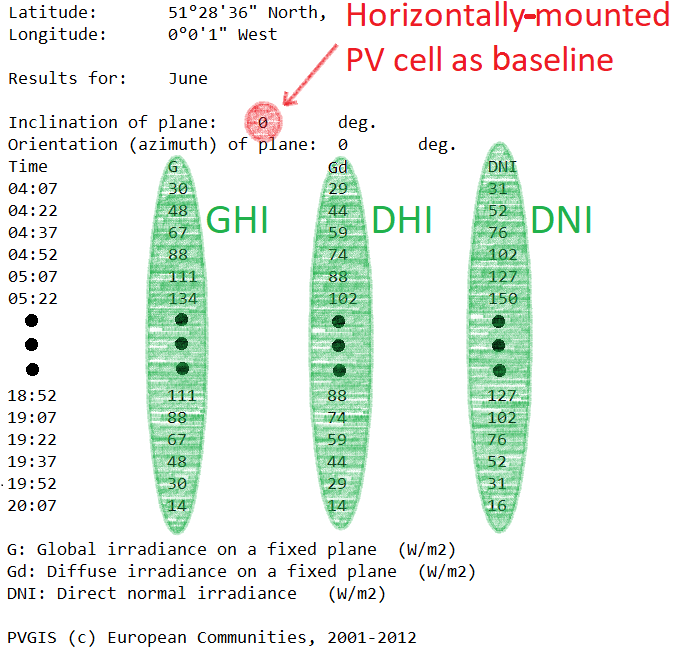
\includegraphics[width=0.7\columnwidth]{pictures/Greenwich5}
\caption[PVGIS data sheet]{PVGIS data sheet from \cite{PVGIS}\label{PVGIS_datasheet}}
\end{figure}

 
The energy generated by one PV cell installed with orientation angle $\theta$ and surface area $\frac{A}{N}$ is denote by $G^{\text{original}}_{\theta,N}(t)$ and can be calculated by \cite{add}\footnote{The total irradiance received by the PV cell $I_{\theta}(t)$ adjusted for angle of incidence losses inside of the PV cell module, for soiling, e.g., dust or snow, for temporal losses, and for spectral mismatch is called the effective irradiance (irradiance that is “available” to the PV cell for power conversion). The material covering a cell in a PV module, e.g., glass, and encapsulate, causes due to reflection and absorption different losses at different angles of incidence. It is out of the scope of this thesis to calculate any internal energy losses of the PV cell due to its structure or composition. Therefore, it is assumed for simplicity that the total irradiance received by the PV cell $I_{\theta}(t)$ is the effective irradiance available by the PV cell for conversion in this thesis.} as follows:

\begin{equation}\label{normalization}
G^{\text{original}}_{\theta,N}(t)=I_{\theta}(t) \cdot \eta \cdot \frac{A}{N} \cdot \tau,
\end{equation}
where $I_{\theta}(t)$ is the irradiance received by the PV cell, $\eta$ is the energy conversion efficiency, $\frac{A}{N}$ is the surface area of the PV cell, and $\tau$ is the duration of one time step.

To facilitate a fair comparison in Section \ref{results}, all energy generation values are normalized with respect to a south-orientated PV cell in Greenwich at noon with surface area $A$, and inclination angle $\gamma=36^{\mathrm{o}}$ (optimal inclination angle for Greenwich (London, UK) in summer). Among all orientation angle settings and among all time steps throughout the day, the peak energy generation occurs during noon when all available PV cells are south-oriented in Greenwich. This is because Greenwich is located on the reference meridian of its time zone. The time step $t=\frac{T}{2}$ is noon. Because a south-orientated PV cell in Greenwich has its peak energy generation at noon, i.e., $I_{0^{\mathrm{o}}}\big(\frac{T}{2}\big)\geq I_{0^{\mathrm{o}}}\big(t\big)\quad \forall t\in\{1,...,T\}$, the peak irradiance value at noon, i.e, $614[\frac{W}{m^2}]=I_{0^{\mathrm{o}}}\big(\frac{T}{2}\big)$, is used as normalization factor in this thesis. The peak irradiance value is derived from \cite{PVGIS} by downloading the data sheet for a south-oriented PV cell in Greenwhich with  inclination angle $\gamma=36^{\mathrm{o}}$. The normalization factor $614$ has the effect that exactly 1 unit of normalized energy is generated by the south-oriented PV cell at noon after normalization. This normalization is done for convenience. Any normalization factor can be used but normalization the peak energy generation to 1 unit of energy is convenient when representing the results in graphs. Other locations than Greenwich (London, UK) will have to use their respective normalization factor and their respective optimal inclination angle. Appendix A will do the normalization process step by step for a better understanding.


Hence, $G_{\theta,N}(t)$ is the normalized energy generated by one PV cell out of the $N$ PV cells installed with orientation angle $\theta$ and can be calculated by

\begin{equation}\label{norma}
G_{\theta,N}(t)=\frac{G_{\theta,N}^{\text{original}}(t)}{G^{\text{original}}_{0^{\mathrm{o}},1}\big(\frac{T}{2}\big)}=\frac{I_{\theta}(t)}{I_{0^{\mathrm{o}}}\big(\frac{T}{2}\big)\cdot N}= \frac{I_{\theta}(t)}{614\cdot N}.
\end{equation}



The normalized energy generated by $N$ PV cells, denoted by $G_{(\theta_1, ..., \theta_N)}(t)$, is calculated as follows:
\begin{equation}\label{nor}
G_{(\theta_1, ..., \theta_N)}(t)=\sum_{i=1}^N G_{\theta_i,N}(t).
\end{equation}

As a result, if all $N$ PV cells are oriented to the south, they generate exactly 1 unit of energy at noon, i.e., $G_{(\theta_1, ..., \theta_N)}\big(\frac{T}{2}\big)=G_{(0^{\mathrm{o}}, ...,0^{\mathrm{o}})}\big(\frac{T}{2}\big)=1$.



The irradiance $I_{\theta}(t)$ received by one PV cell installed with orientation angle $\theta$ at time step $t$ can be calculated by \cite{Solar_Cell_3irradiance} as follows:


\begin{equation}\label{I1}
I_{\theta}(t)=I_{b_\theta}(t)+I_{d_\theta}(t)+I_{g}(t),
\end{equation}
where $I_{b_\theta}(t)$ is the direct-beam component, $I_{d_\theta}(t)$ is the sky-diffuse component, and $I_{g}(t)$ is the ground-reflected component. Figure \ref{3irradiances} shows the three components graphically. The three irradiance components are investigated in the next three sections separately.

\begin{figure}[H]
	\centering
		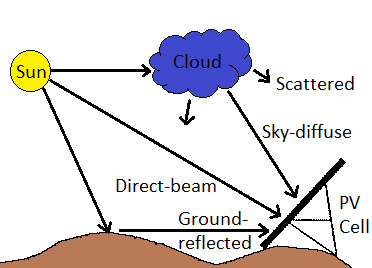
\includegraphics[width=0.6\columnwidth]{pictures/3irradiances}
\caption{Irradiance model\label{3irradiances}}
\end{figure}



\subsection{Ground-reflected Irradiance \texorpdfstring{$I_g(t)$}{I\_g(t)}}\label{ground_reflected_component}

The ground-reflected irradiance $I_{g}(t)$ is independent of the orientation angle $\theta$ and can be calculated by \cite{Solar_Cell_albedo_plus_ground_reflected_irradiance} as follows:


\begin{equation}\label{I3}
I_{g}(t)= GHI_t \cdot \alpha \cdot \frac{1-\cos(\gamma)}{2},
\end{equation}
where $\alpha\in[0,1]$ is the albedo of the ground. The albedo is dimensionless and measures the amount of sunlight that a surface reflects. A black body that absorbs all sunlight has an albedo value of $0$. A body that reflects all sunlight has an albedo value of $1$. For example, snow has a high albedo and hence, appears bright. Trees have a low albedo and hence, appear dark.



\subsection{Direct-beam Irradiance \texorpdfstring{$I_{b_\theta}(t)$}{I\_{b\_{\{theta\}}}(t)}}\label{direct_beam_component}
The direct-beam irradiance $I_{b_\theta}(t)$ depends on the orientation angle $\theta$ and can be calculated by \cite{Solar_Cell_3irradiance} as follows:


\begin{equation}\label{I4}
I_{b_\theta}(t)=DNI_t \cdot  \max(0,\cos(AOI_{\theta}(t))),
\end{equation}
where $AOI_{\theta}(t)$ is the angle of incidence at time step $t$.

It is important to include the $\max$ in (\ref{I4}) to model that no energy can be harvest if the PV cell is illuminated from the back, i.e., $AOI_{\theta}(t)>90^\mathrm{o}$. For example, if the PV cell is oriented to the east then $AOI_{\theta}(t)$ will be greater than $90^\mathrm{o}$ in the evening. Hence, $\cos(AOI_{\theta}(t))$ will be smaller than $0$. This will result in a negative irradiance value $I_{b_\theta}(t)$ during the evening, which makes no sense. As a result, the $\max$ in (\ref{I4}) is necessary.

The angle of incidence $AOI_{\theta}(t)$ is the angle between the line that points to the sun and the normal vector to the PV cell panel (cf. Figure \ref{AOI}). $AOI_{\theta}(t)$ can be calculated by \cite{Solar_Cell_declination_inclination_angle} as follows:

\begin{align}
\cos(AOI_{\theta}(t))= &\quad \textcolor{SeaBlue}{+ \sin(\delta_d) \sin(lat) \cos(\gamma)} \nonumber \\
					 &\quad \textcolor{SeaBlue}{+ \cos(\delta_d) \cos(lat) \cos(\gamma) \cos(\omega_t)} \nonumber \\
			   	 &\quad \textcolor{Orange8}{+ \cos(\delta_d) \sin(\gamma) \sin(\omega_t)} \!\!\enskip \textcolor{red!70}{ \sin(\theta)} \nonumber \\
					 &\quad \textcolor{Gray7}{- \sin(\delta_d) \cos(lat) \sin(\gamma)} \!\!\enskip \textcolor{red}{ \cos(\theta)} \nonumber \\
					 &\quad \textcolor{Gray7}{+ \cos(\delta_d) \sin(lat) \sin(\gamma) \cos(\omega_t)} \!\!\enskip \textcolor{red}{ \cos(\theta)} \label{allgemein_AOI}\\
					= &\quad \textcolor{SeaBlue}{a_t} +\textcolor{Orange8}{b_t} \textcolor{red!70}{\sin(\theta)} + \textcolor{Gray7}{c_t} \textcolor{red}{\cos(\theta)}, \text{ with}\nonumber 
\end{align}




\begin{align}
\textcolor{SeaBlue}{a_t}=&\quad \textcolor{SeaBlue}{+ \sin(\delta_d) \sin(lat) \cos(\gamma)}\nonumber  \\
					               &\quad \textcolor{SeaBlue}{+ \cos(\delta_d) \cos(lat) \cos(\gamma) \cos(\omega_t)}, \label{a_t}\\
\textcolor{Orange8}{b_t}=&\quad \textcolor{Orange8}{+ \cos(\delta_d) \sin(\gamma) \sin(\omega_t)} \label{b_t},\\
  \textcolor{Gray7}{c_t}=&\quad \textcolor{Gray7}{- \sin(\delta_d) \cos(lat) \sin(\gamma)} \nonumber  \\
					               &\quad \textcolor{Gray7}{+ \cos(\delta_d) \sin(lat) \sin(\gamma) \cos(\omega_t)}, \label{c_t}
\end{align}
where $lat$ is the latitude of the deployment area, $\delta_d$ is the declination angle, and $\omega_t$ is the hour angle at time step $t$. $a_t$, $b_t$, and $c_t$ include the parts that are independent of $\theta$, are multiplied by $\sin(\theta)$, and are multiplied by $\cos(\theta)$, respectively.
\begin{figure} [H]
	\centering
		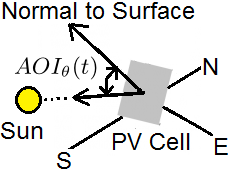
\includegraphics[width=0.3\textwidth]{pictures/AOI2}
		\caption{Definition of the angle of incidence $AOI_{\theta}(t)$\label{AOI}}
\end{figure}
The declination angle $\delta_d$ can be calculated by \cite{Solar_Cell_declination} as follows:


\begin{equation} \label{delta}
\delta_d=23.45^\mathrm{o} \cdot \sin\left(\frac{360}{365} (d+284)\right),
\end{equation}


where $d$ is the day of the year with $1^{\mathrm{st}}$ of January as $d = 1$.

The declination angle models the different seasons (cf. Figure \ref{decli}). $23.45^{\mathrm{o}}$ is the axial tilt of the earth.


\begin{figure}[H]
	\centering
		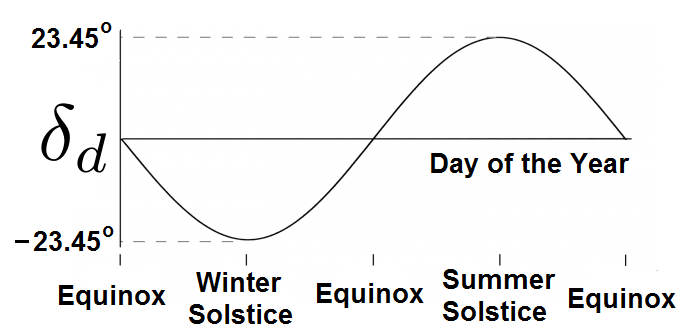
\includegraphics[width=0.6\columnwidth]{pictures/decli}
\caption{Declination angle $\delta_d$ throughout the year\label{decli}}
\end{figure}


The hour angle $\omega_t$ is defined as the angle between the meridian that intersects with the line that points to the sun and the meridian containing the observer (cf. Figure \ref{hour_angle}). 
The hour angle $\omega_t$ is depicted for Greenwich (London, UK) in Figure \ref{hour_angle_graph}. Because Greenwich (London, UK) is located on the reference meridian of its time zone, the straight line in Figure \ref{hour_angle_graph} intersects the x-axis at noon\footnote{The hour angles $\omega_t$ of locations that are not on their reference meridian of their time zone can be depicted by a straight line as well which is shifted along the x-axis. The formula to calculate the x-axis shift is given in \cite{Solar_Cell_hour_angle}.}. $\omega_t$ has a period of 24 hours and ranges from $-180^{\mathrm{o}}$ to $180^{\mathrm{o}}$.




\begin{figure} [H]
	\centering
		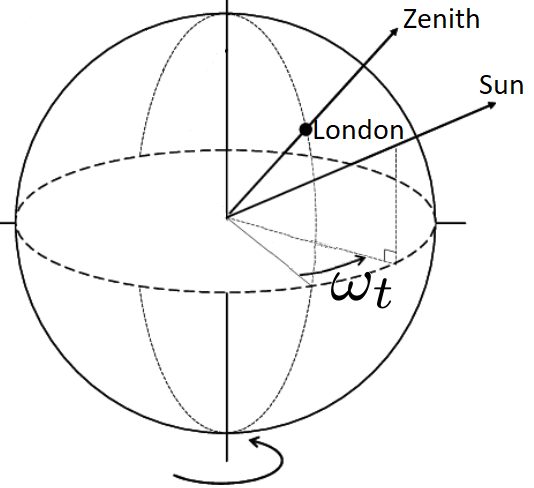
\includegraphics[width=0.3\textwidth]{pictures/hour_angle}
		\caption{Definition of the hour angle $\omega_t$\label{hour_angle}}
\end{figure}



\begin{figure}[H]
	\centering
		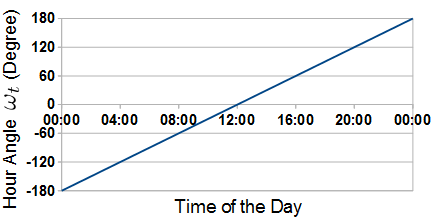
\includegraphics[width=0.6\columnwidth]{pictures/hour_angle_graph}
\caption{Hour angle $\omega_t$ throughout the day of a PV cell located on the reference meridian of its time zone \label{hour_angle_graph}}
\end{figure}


\subsection{Sky-diffuse Irradiance \texorpdfstring{$I_{d_\theta}(t)$}{I\_{d\_\{theta\}}(t)}}\label{sky_diffuse_component}
The sky-diffuse irradiance $I_{d_\theta}(t)$ is derived from the Reindl model\footnote{The difference between different irradiance models are usually in the way they model the sky-diffuse irradiance \cite{different_irradiance_model,DemainColienne2013Eodm,BertrandCdric2015Eodm}. The simplest and most commonly used model is the Liu and Jordan model, which assumes an isotropic diffuse sky \cite{irradianceModels}. In other words, the diffuse-sky irradiance is uniform across the sky and hence, the diffuse-sky irradiance is independent of the orientation angle $\theta$. The more advanced Reindl model is used in this thesis \cite{GueymardChristianA.2009Daiu}, which breaks the diffuse-sky irradiance into three separate parts: the isotropic component, the circumsolar component, and the horizon brightening component. The first component is the same as the Liu and Jordan model, while the other components are small correction terms. The circumsolar component dependents on the orientation angle $\theta$.} \cite{reindl,diffuse} as follows:

\footnotesize


\begin{align}\label{reindl}
I_{d_\theta}(t)=&\underbrace{DHI_t\cdot\vphantom{\sqrt(\frac{(X)^x_x}{(X)^x_x})}A_t\cdot \frac{\max(0,\cos(AOI_{\theta}(t)))}{\cos(\zeta_t)}}_{\text{Circumsolar Component}}+\underbrace{DHI_t\cdot(1-A_t)\cdot\frac{1+\cos(\gamma)}{2}}_{\text{Isotropic Component}}+\nonumber\\
&\underbrace{DHI_t\cdot(1-A_t)\cdot\frac{1+\cos(\gamma)}{2} \cdot\sqrt{\frac{DNI_t\cdot \cos(\zeta_t)}{GHI_t}}\sin^3\bigg(\frac{\gamma}{2}\bigg)}_{\text{Horizon Brightening Component}}=\nonumber\\
DHI_t\bigg[\vphantom{\sqrt(\frac{(X)^x_x}{(X)^x_x})}&A_t\cdot \frac{\max(0,\cos(AOI_{\theta}(t)))}{\cos(\zeta_t)}+(1-A_t)\cdot\frac{1+\cos(\gamma)}{2}\cdot\bigg(\vphantom{\sqrt(\frac{(X)^x_x}{(X)^x_x})}1+\sqrt{\frac{DNI_t\cdot \cos(\zeta_t)}{GHI_t}}\sin^3\bigg(\frac{\gamma}{2}\bigg)\bigg)\bigg],\nonumber\\
\end{align}
\normalsize
where $A_t$ is the anisotropy index, and $\zeta_t$ is the solar zenith angle. The Reindl model breaks the diffuse-sky irradiance into three separate parts: the isotropic component, the circumsolar component, and the horizon brightening component (cf. (\ref{reindl})). The circumsolar component depends on the orientation angle $\theta$. The isotropic component, and the horizon brightening component do not depend on the orientation angle $\theta$.



The solar zenith angle $\zeta_t$ can be calculated by \cite{zenith_angle} as follows:


\begin{equation}\label{zenith}
\cos(\zeta_t)=\sin(lat)\sin(\delta_d)+\cos(lat)\cos(\delta_d)\cos(\omega_t).
\end{equation}


The anisotropy index $A_t$ of time step $t$ can be calculated by \cite{reindl} as follows:


\begin{equation} \label{At}
A_t=\frac{DNI_t}{E_d},
\end{equation}

\noindent
where $E_d$ is the extraterrestrial radiation. It can be calculated by \cite{Ea} as follows:


\begin{equation}\label{extra}
E_d=E_{\mathrm{con}}\cdot \bigg(\frac{\overline{r}}{r_d}\bigg)^2=E_{\mathrm{con}}\cdot\bigg(1+0.033 \cdot \cos \bigg(\frac{360 \cdot d}{365}\bigg)\bigg),
\end{equation}
where $E_{\mathrm{con}}$ is the solar constant set at $1367 \frac{\mathrm{W}}{\mathrm{m}^2}$ \cite{Solar_Cell_declination_inclination_angle}, $\overline{r}$ is the mean sun-earth distance also called $1$ astronomical unit ($1$ AU), $r_d$ is the actual sun-earth distance, which depends on the day of the year, and $d$ is the day of the year with $1^{\mathrm{st}}$ of January as $d = 1$.




\subsection{Energy Consumption of a BS\label{consumption}}


$C^{\text{original}}(t)$ is the original energy consumption by the BS during time step $t$ ($\tau$ is the duration of one time step) and $C(t)$ is the normalized energy consumption by the BS at time step $t$ and can be calculated by

\begin{equation}
C(t)=\frac{C^{\text{original}}(t)}{G^{\text{original}}_{0^{\mathrm{o}},1}\big(\frac{T}{2}\big)},
\end{equation}

where $G^{\text{original}}_{0^{\mathrm{o}},1}\big(\frac{T}{2}\big)$ is the peak energy generation of the PV cells if they are all south-oriented at noon.
A practical example is given in Appendix A to show step by step the process of normalization. 

$C(t)$ consists of a load-dependent part and a load-independent part. Three different load scenarios are investigated: a BS deployed with constant traffic load $C_{\mathrm{con}}(t)$, with business-area traffic load $C_{\mathrm{bus}}(t)$, and with residential-area traffic load $C_{\mathrm{res}}(t)$ (cf. Figure \ref{all_consumption_profiles}). Three different example energy consumption profiles are given to show the composition of C(t) into a load-dependent part and a load-independent part as follows:

\begin{align}
&C(t)=\underbrace{C_{\mathrm{con}}(t)}_{\text{load-dependent part}} + \underbrace{1}_{\text{load-independent part}}\\
&C(t)=\underbrace{C_{\mathrm{bus}}(t)}_{\text{load-dependent part}} + \underbrace{0.2}_{\text{load-independent part}}\\
&C(t)=\underbrace{C_{\mathrm{res}}(t)}_{\text{load-dependent part}} + \underbrace{0.7}_{\text{load-independent part}}.
\end{align}

The load-dependent part of the energy consumption profile determines the shape of the energy consumption profile, i.e., whether there is one significant peak in the profile, or several significant peaks in the profile or a very flat profile without any peaks.

The exact values for $C_{\mathrm{con}}(t)$, $C_{\mathrm{bus}}(t)$, and $C_{\mathrm{res}}(t)$ are given in Appendix B "Input File (Load Profiles)" for all time steps $t\in\{1,...,T\}$ as well as in Figure \ref{all_consumption_profiles}.
It can be observed that the traffic load in a business area ($C_{\mathrm{bus}}(t)$) is significantly higher during business hours than the rest of the day, while it drops a bit during lunch hours. Hence, there is one significant peak in the business area traffic load profile during afternoon hours. The traffic load in a residential area ($C_{\mathrm{res}}(t)$) is anti-correlated to the traffic load in a business area because it is higher during times when people are usually not working with its peak during late evening. This profile has peaks in the morning as well as in the evening.




\begin{figure}[H]
	\centering
		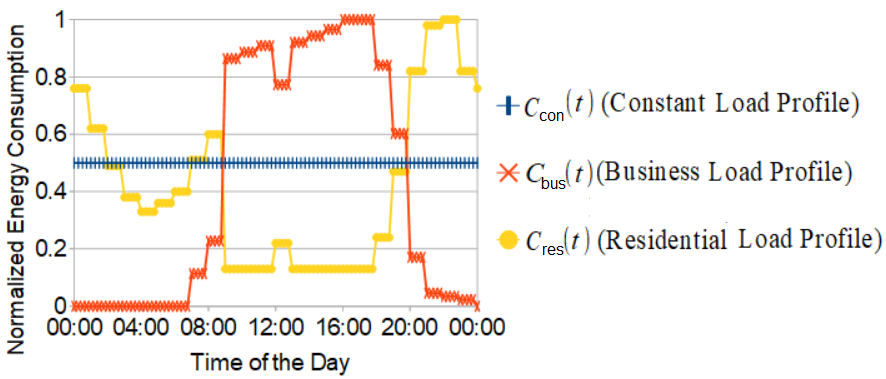
\includegraphics[width=0.8\columnwidth]{pictures/all_consumption_profiles2}
\caption[Constant traffic load profile, business traffic load profile, and residential traffic load profile throughout the day]{Constant traffic load profile, business traffic load profile, and residential traffic load profile throughout the day. Data source: \cite{load}\label{all_consumption_profiles}}
\end{figure}

For each of the three different load scenarios, I want to investigate how the relationship between the energy generation profile and the energy consumption profile affects the outcome of the orientation angles optimization. Therefore, I choose different values for the load-independent part of the energy consumption so that I have a case study in which the energy generation is significantly greater than the energy consumption ($G>>C$), the energy generation is slightly greater than the energy consumption ($G>C$), the energy generation is slightly smaller than the energy consumption ($G<C$), and the energy generation is significantly smaller than the energy consumption ($G<<C$). Figures \ref{constant_allgemein} - \ref{residential_allgemein} show all energy consumption profiles $C(t)$ which will be numerically investigated in section \ref{results}. The energy consumption profiles with the highest load-independent part in each figure belongs to the category $G<<C$. The energy consumption profiles with the lowest load-independent part in each figure belongs to the category $G>>C$.



To see the relationships between the energy consumption profiles $C(t)$ and the energy generation profiles $G(t)$, the combined energy generation profile of two south-oriented PV cells $G_{(0^\mathrm{o},0^\mathrm{o})}(t)$ as well as the combined energy generation profile of an east-oriented PV cell with a west-oriented PV cell $G_{(-90^\mathrm{o},90^\mathrm{o})}(t)$ are shown. 



\begin{figure}[H]
	\centering
		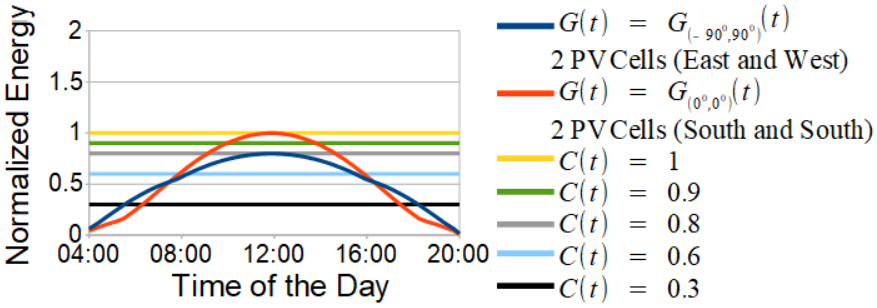
\includegraphics[width=1\columnwidth]{pictures/constant_allgemein3}
\caption{Energy consumption profiles with constant traffic load and energy generation profiles of 2 PV cells\label{constant_allgemein}}
\end{figure}


\begin{figure}[H]
	\centering
		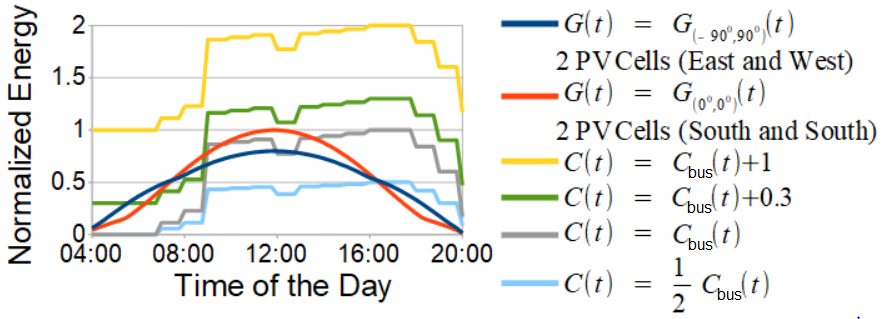
\includegraphics[width=1\columnwidth]{pictures/business_allgemein3}
\caption{Energy consumption profiles with business-area traffic load and energy generation profiles of 2 PV cells\label{business_allgemein}}
\end{figure}

\begin{figure}[H]
	\centering
		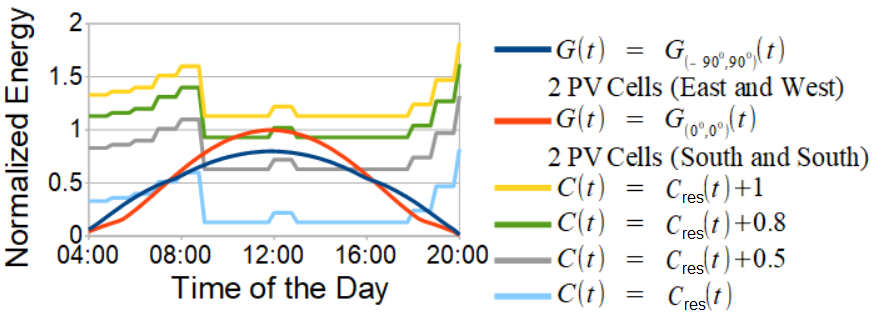
\includegraphics[width=1\columnwidth]{pictures/residential_allgemein3}
\caption{Energy consumption profiles with residential-area traffic load and energy generation profiles of 2 PV cells\label{residential_allgemein}}
\end{figure}




\subsection{Problem Formulation \label{generalization}}
The optimization objective is to minimize the normalized energy drawn from the main grid $f(\theta_1, ..., \theta_N)$ by the BS throughout the day which is defined in (\ref{optimization_objective}). The optimization problem is formulated as follows:

\begin{align}
f(\theta_1, ..., \theta_N)&=\sum_{t=1}^T \max\{0, C(t)-G_{(\theta_1, ..., \theta_N)}(t)\} \label{optimization_objective}\\
(\theta_1^*, ..., \theta_N^*)&=\arg \underset{(\theta_1, ..., \theta_N)}{\min}f(\theta_1, ..., \theta_N) \label{optimization_objective1},
\end{align}
where $(\theta_1^*, ..., \theta_N^*)$ are the optimal orientation angles for the $N$ PV cells.




Because surplus energy is wasted or fed to the grid with no feed-in tariff in the system model 1, the maximum out of  $0$ and $C(t) - G_{(\theta_1, ..., \theta_N)}(t)$ has to be taken in (\ref{optimization_objective}). It is assumed that energy can be bought from the grid at a fixed price throughout the day (flat rates). Hence, the objective function is to minimize the accumulated energy deficit throughout the day in (\ref{optimization_objective})-(\ref{optimization_objective1}). $f(\theta_1, ..., \theta_N)$ is transformed in (\ref{be}) - (\ref{intermit}). Eq. (\ref{intermit}) is used in Appendix B.




\begin{align}
f(&\theta_1, ..., \theta_N)=\sum_{t=1}^T \max\left\{0, C(t)-\sum_{n=1}^N G_{\theta_n,N}(t)\right\}\label{be}\\
&= \sum_{t=1}^T \max\bigg\{0, \underbrace{C(t)-\frac{I_{g}(t)}{614}}_{I_{\text{fix}}(t)}-\sum_{n=1}^N \frac{I_{b_{\theta_n}}(t)+I_{d_{\theta_n}}(t)}{{614}\cdot N}\bigg\}\\
&= \sum_{t=1}^T \max\bigg\{0,I_{\text{fix}}(t)-\sum_{n=1}^N \frac{I_{b_{\theta_n}}(t)+I_{d_{\theta_n}}(t)}{{614}\cdot N}\bigg\}\label{intermit}
\end{align}


The gain $\Delta_n$ of adding the $n^{\mathrm{th}}$ PV cell with optimal orientation angle $\theta_n^*$ to the system model 1 is defined as follows:


\begin{equation} \label{Delta_n}
\Delta_n=f(\theta_1^*,...,\theta_{n-1}^*)-f(\theta_1^*,...,\theta_n^*),\quad n\in \{2, ..., N\}.
\end{equation}


The gain of adding the first PV cell with optimal orientation angle $\theta_1^*$ to the system model 1 is defined as follows:

\begin{equation}\label{Delta_1}
\Delta_1=f(0^\mathrm{o})-f(\theta_1^*).
\end{equation}


A positive (negative) $\Delta_n$ value represents an improvement (deterioration) in performance of the system if the $n^{\mathrm{th}}$ PV cell is added, $n\in\{1, ..., N\}$.

\section{Analytical Insights obtained from Section \ref{system_1}\label{analytical}}
This section identifies and discusses analytically to what extent the orientation angle $\theta$ shifts the energy generation profile away from noon if the PV cells are not south-oriented ($\theta \neq 0^\mathrm{o}$). The direct-beam irradiance $I_{b_\theta}(t)$ and the sky-diffuse irradiance  $I_{d_\theta}(t)$ depend on $\theta$. Nonetheless, because the
main component of the sky-diffuse irradiance is independent of $\theta$ (isotropic component), while the other two components, which are dependent on $\theta$, are small correction terms, the focus will be on the direct-beam irradiance in this section.

Figure \ref{abc_values} shows the values of $a_t$, $b_t$, and $c_t$ throughout one day for the spring equinox ($d=81$), summer solstice ($d=172$), autumn equinox ($d=264$), and winter solstice ($d=355$). $\gamma$ is fixed to $36^{\mathrm{o}}$, and the location to Greenwich ($lat=51.4767^{\mathrm{o}}$ North, $lon=0.0003^{\mathrm{o}}$ West) to calculated the $a_t$, $b_t$, and $c_t$ values. Only the hour angle $\omega_t$ changes throughout the day, whereas all other parameters are constant throughout the day in (\ref{a_t}) - (\ref{c_t}). Therefore, $a_t$, $b_t$, and $c_t$ have a sine or cosine behavior with the y-axis shifts and amplitudes are summarized in (\ref{allgemein_AOI3}) - (\ref{allgemein_AOI4}). Because $w_t$ has a period of 24 hours, $a_t$, $b_t$, and $c_t$ have a period of 24 hours as well. 
The only angle that changes for different seasons is $\delta_d$ because it depends on the day of the year $d$. Therefore, the differences between the four $a_t$ curves, the four $b_t$ curves as well as the four $c_t$ curves are caused only by $\delta_d$. The curves for the spring equinox and autumn equinox are identical, i.e., $a_t$ ($d=81$) = $a_t$ ($d=264$), $b_t$ ($d=81$) = $b_t$ ($d=264$), and $c_t$ ($d=81$) = $c_t$ ($d=264$). 



\begin{align}
a_t =& \quad \textcolor{SeaBlue}{\underbrace{+\sin(\delta_d) \sin(lat) \cos(\gamma)}_{\text{y-axis shift}}} \nonumber\\
     & \quad\textcolor{SeaBlue}{\underbrace{+\cos(\delta_d) \cos(lat) \cos(\gamma)}_{\text{amplitude}} \cos(\textcolor{red}{\omega_t})} \label{allgemein_AOI3}\\
		b_t =& \quad \textcolor{Orange8}{\underbrace{+\cos(\delta_d) \sin(\gamma)}_{\text{amplitude}}\sin(\textcolor{red}{\omega_t})} \\      
c_t =& \quad \textcolor{Gray7}{\underbrace{-\sin(\delta_d) \cos(lat) \sin(\gamma)}_{\text{y-axis shift}}}\nonumber\\
     & \quad\textcolor{Gray7}{\underbrace{+\cos(\delta_d) \sin(lat) \sin(\gamma)}_{\text{amplitude}} \cos(\textcolor{red}{\omega_t})}\label{allgemein_AOI4} 
\end{align}


\begin{figure}[H]
	\centering
		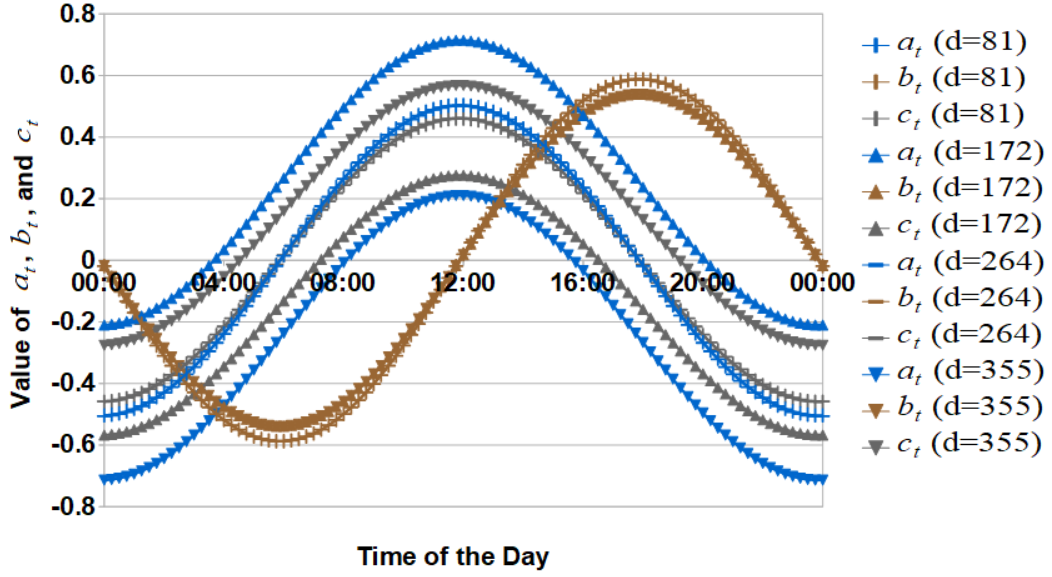
\includegraphics[width=1\columnwidth]{pictures/abc}
\caption[Values of $a_t$, $b_t$, and $c_t$ throughout one day for the spring equinox, summer solstice, autumn equinox, and winter solstice]{Values of $a_t$, $b_t$, and $c_t$ throughout one day for the spring equinox ($d=81$), summer solstice ($d=172$), autumn equinox ($d=264$), and winter solstice ($d=355$). $\gamma$ is set at $36^{\mathrm{o}}$, and the location is Greenwich ($lat=51.4767^{\mathrm{o}}$ North, $lon=0.0003^{\mathrm{o}}$ West) for all scenarios.  \label{abc_values}}
\end{figure}



The following insights are obtained from (\ref{allgemein_AOI3}) to (\ref{allgemein_AOI4}):

\begin{itemize}
\item $a_t$ and $c_t$ are symmetrical to noon. Hence, if $\theta\neq 0^\mathrm{o}$, i.e., $\sin(\theta)\neq 0$, $b_t$ is solely responsible for shifting the energy generation peak towards the morning or afternoon hours. If $\theta$ is orientated eastwards (westwards), then $\theta<0^{\mathrm{o}}$ ($\theta>0^{\mathrm{o}}$), and $\sin(\theta)< 0$ ($\sin(\theta)> 0$), and hence the energy generation peak is shifted toward the morning (afternoon) hours.
\item Also (\ref{I4}) causes an asymmetric energy generation profile if $\theta\neq0^{\mathrm{o}}$. The $\max$ in (\ref{I4}) removes the direct-beam irradiance if the PV cell is illuminated from the back. The more the PV cell is orientated eastwards (westwards), the longer the PV cell is illuminated from the back in the evening (morning) and the more energy is lost in the evening (morning).
\item If the location of the PV cell is on the equator, the PV cell should be installed with the default inclination angle $\gamma=0^\mathrm{o}$ (cf. Table \ref{over}). As a consequence, $\sin(\gamma)=0$, and $b_t=c_t=0$. As a result, any orientation angle can be chosen for a PV cell on the equator because the orientation angle does not affect the energy generation profile of a PV cell on the equator. Figure \ref{fig:June} provides graphically the proof by using the data from PVGIS \cite{PVGIS}.
Hence, orientation angle optimization should be done for PV cells a bit farther away from the equator, where PV cells are not horizontally mounted. Alternatively, PV cells on the equator can be inclined ($\gamma\neq 0^\mathrm{o}$) a bit to facilitate orientation angle optimization at the cost of reducing the average daily energy yield of the PV cells.

\begin{figure}[H]
	\centering
		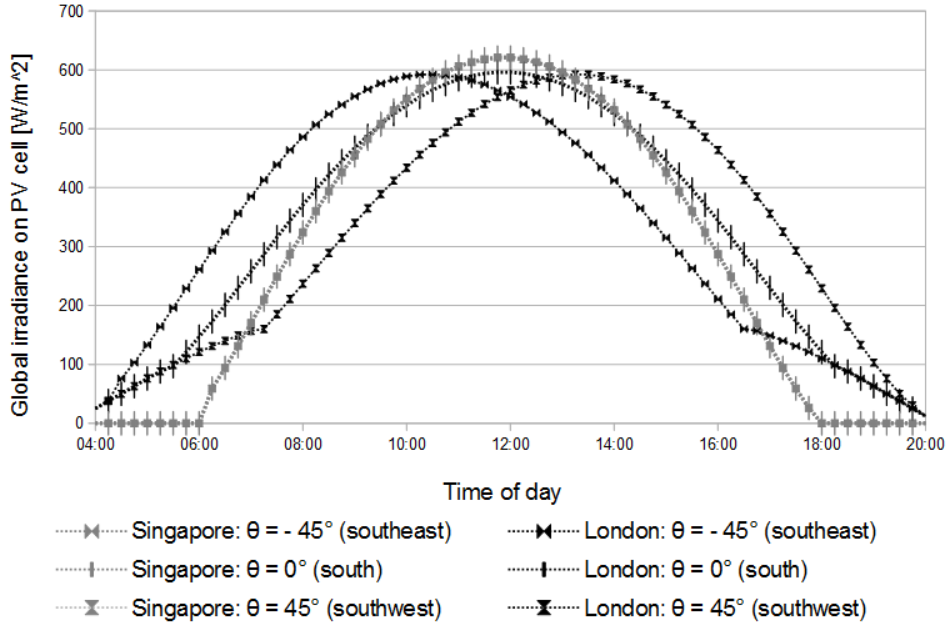
\includegraphics[width=\columnwidth]{pictures/lon-sin}
\caption[Irradiance values of differently oriented PV cells in Greenwich (London, UK) and Singapore]{Irradiance values of differently orientated PV cell installations in Greenwich (temperate zone on northern hemisphere) and Singapore (close to equator) in June. An inclination angle of $38^{\mathrm{o}}$ ($0^{\mathrm{o}}$) was chosen for Greenwich (Singapore).\\ Data source: \cite{PVGIS} \label{fig:June}}

\end{figure}
\item The amplitude of $b_t$ is equal to the amplitude of $c_t$ at the north and south poles, whereas the amplitude of $b_t$ is greater than the amplitude of $c_t$ at any other location. 
\end{itemize}



\section{Results and Discussion\label{results}}
Table \ref{tab:inpu_1} summarizes all parameters and their values. 
The total surface area of the $N$ PV cells, denoted by $A$, the duration of one time step, denoted by $\tau$, and the energy conversion efficiency of the PV cells, denoted by $\eta$, do not appear in (\ref{norma}) anymore due to the normalization of the energy generation in (\ref{norma}). As a result, there is no value assigned to these parameters in Table \ref{tab:inpu_1}.

The derived $I_{\theta}(t)$ values in this thesis were compared with the modeled irradiance values from the PVGIS database (daily data profiles \cite{tool}). Both values were the same. This proves that our derivation and implementation of the irradiance model is correct. The irradiance model implemented in PVGIS \cite{PVGIS} is the Muneer model \cite{muneer}, but it is mentioned on the PVGIS website \cite{method} that the Muneer model performs very similar to the Reindl model. The Reindl model was used in this thesis. 


\begin{longtable}{@{}l*{2}{|l}l@{}}
\caption{\\ Input parameters of system model 1\label{tab:inpu_1}}\\ \toprule
\textbf{Parameter}	&\textbf{Description}				&  \textbf{Value} \\ \midrule
$\alpha$  &Albedo of ground&$0.2$ (Grassland)\\
$\gamma$  &Inclination angle &$36^{\mathrm{o}}$\\
$\delta_d$ &Declination angle & Eq. (\ref{delta})\\
$\zeta_t$  &Zenith angle & Eq. (\ref{zenith})\\
$\eta$  &Energy conversion efficiency of the PV cells & \\
$\theta$  &Orientation angle&$\in [-90^{\mathrm{o}},90^{\mathrm{o}}]$\\
$\theta_1, ..., \theta_N$ &Orientation angles of PV cells $1,..., N$&$\in [-90^{\mathrm{o}},90^{\mathrm{o}}]$\\
$\theta_1^*, ..., \theta_N^*$ &Optimal orientation angles $\theta_1, ..., \theta_N$ &$\in [-90^{\mathrm{o}},90^{\mathrm{o}}]$\\
$\tau$ & Duration of one time step& \\
$\omega_t$ &Hour angle&Figure \ref{hour_angle_graph}\\
$\Delta_1$ &Gain of adding the $1^{\mathrm{st}}$ PV cell&Eq. (\ref{Delta_1})\\
$\Delta_n$ &Gain of adding the $n^{\mathrm{th}}$ PV cell, $n\in\{2, ..., N\}$&Eq. (\ref{Delta_n})\\
$A$ & Total surface area of $N$ PV cells& \\
$A_t$ &Anisotropy index at time step $t$&Eq. (\ref{At}) \\
$AOI_{\theta}(t)$ &Angle of incidence &Eq.  (\ref{allgemein_AOI})\\
$C(t)$ &Energy consumption of BS at time step $t$ &Figures \ref{constant_allgemein} - \ref{residential_allgemein}\\
$C_{\mathrm{bus}}(t)$ & Business-area traffic load profile at time step $t$& Figure \ref{all_consumption_profiles}\\
$C_{\mathrm{con}}(t)$ & Constant traffic load profile at time step $t$&Figure \ref{all_consumption_profiles}\\
$C_{\mathrm{res}}(t)$ &  Residential-area traffic load profile at time step $t$&Figure \ref{all_consumption_profiles}\\
$DHI_t$ &Diffuse horizontal irradiance at time step $t$&PVGIS \cite{PVGIS} \\
$DNI_t$ &Direct normal irradiance at time step $t$  &PVGIS \cite{PVGIS} \\
$E_d$ & Extraterrestrial radiation &Eq. (\ref{extra}) \\
$E_{\mathrm{con}}$ & Solar constant &$1367\frac{\mathrm{W}}{\mathrm{m}^2}$ \cite{Solar_Cell_declination_inclination_angle}\\
$G(t)$ &Energy generation of PV cell/cells at time step $t$& \\
$G^{\text{original}}_{\theta,N}(t)$&Energy generated by one&\\
&PV cell installed with $\theta$ at time step $t$&\\
&($N$ is the total number of PV cells)&Eq. (\ref{normalization})\\
$G_{\theta,N}(t)$ &Normalized energy generated by&\\
& one PV cell installed with $\theta$ at time step $t$&\\
&($N$ is the total number of PV cells)&Eq. (\ref{norma})\\
$G_{(\theta_1, ..., \theta_N)}(t)$ &Normalized total energy&\\
& generated by $N$ PV cells at time step $t$&\\
&installed with $\theta_1, ....,\theta_N$&Eq. (\ref{nor})\\
$GHI_t$ &Global horizontal irradiance at time step $t$  &PVGIS \cite{PVGIS} \\
$I_{\theta}(t)$  &Irradiance on PV cell installed &\\
  & with $\theta$ at time step $t$&Eq. (\ref{I1})\\
$I_{b_\theta}(t)$ &Direct-beam irradiance at time step $t$&Eq.  (\ref{I4})\\
$I_{d_\theta}(t)$ &Sky-diffuse irradiance at time step $t$&Eq.  (\ref{reindl})\\
$I_{g}(t)$ &Ground-reflected irradiance at time step $t$&Eq.   (\ref{I3})\\ 
$N$ &Number of PV cells &$\in \{1,2,3\}$\\
$T$ &Number of time steps&96\\
$a_t$& Independent of $\theta$& Eq. (\ref{a_t})\\
$b_t$& Multiplied by  $\sin(\theta)$ &Eq.  (\ref{b_t})\\
$c_t$& Multiplied by  $\cos(\theta)$&Eq.  (\ref{c_t})\\
$d$ &Day of the year &165 (June)\\
$f(\theta_1, ..., \theta_N)$ &Optimization objective &Eq.  (\ref{optimization_objective})\\
$lat$ &Latitude  &$51.4767^{\mathrm{o}}$ North\\
 &  & (Greenwich)\\
$lon$ &Longitude &$0.0003^{\mathrm{o}}$ West\\
 &&(Greenwich)\\
\bottomrule
\end{longtable}



\subsection{Remarks on the Presentation of the Results\label{results_load_shape}}
The optimal orientation angle(s) will be investigated for 1, 2, and 3 PV cell(s) in Subsections \ref{results_1PV}, \ref{results_2PV}, and \ref{results_3PV}, respectively. The optimal orientation angle will be obtained for each PV cell in the complete range from $- 90^\mathrm{o}$ to $90^\mathrm{o}$ with an angular resolution of $1^\mathrm{o}$.

The graphs in the Table \ref{table_1PV}, Table \ref{table_2PV}, and Table \ref{table_3PV} are generated with MATLAB. The source code of Chapter \ref{Chapter_1} is given in the Appendix B of this thesis and is available on GitHub \cite{DOBEN_GITHUB}.


Normalized energy generation and consumption profiles are used in this thesis. That means the given recommendations in this section can be scaled up for the intended application in the real world. For example, if the derived recommendation for the normalized consumption profile $C(t)$ is to deploy one PV cell with optimal orientation angel $\theta_1^*$,  
that means to deploy several PV cells with the same orientation angle $\theta_1^*$ in the real world if $C(t)$ was the consumption profile of a large-scale BS. Another example, if the derived recommendation for the normalized consumption profile $C(t)$ is to deploy two PV cells with jointly optimized orientation angles $\theta_1^*$ and $\theta_2^*$, that means to deploy several PV cells where half of them are deployed with $\theta_1^*$ and the other half with $\theta_2^*$ in the real world if $C(t)$ was the consumption profile of a large-scale BS. 


\subsubsection{Results for 1 PV Cell (N=1) \label{results_1PV}}

Table \ref{table_1PV} and Table \ref{opt_1PV} show the results for 1 PV cell.

The orientation angle is optimized for three different types of load profiles: the constant load profile $C_{\mathrm{con}}(t)$, the business load profile $C_{\mathrm{bus}}(t)$, and the residential load profile $C_{\mathrm{res}}(t)$ (cf. Figure \ref{all_consumption_profiles}). The left, middle, and right columns in Table \ref{table_1PV} represent the constant, business, and residential load profiles, respectively. Each row in Table \ref{table_1PV} represents the relative relationship between the energy generation profile and energy consumption profile. In other words, the first, second, third, and fourth rows in Table \ref{table_1PV} represent the scenario that the energy generation is significantly smaller, is slightly smaller, is slightly greater, is significantly greater than the energy consumption, denoted by $G<<C$, $G<C$, $G>C$, and $G>>C$, respectively. The red lines in Table \ref{table_1PV} are the optimal orientation angles.

\newpage

\newcounter{tablemajor}
\renewcommand\thetable{\arabic{tablemajor}.\arabic{table}}
\newcommand*\settablecounter[2]{%
        \setcounter{tablemajor}{#1}%
        \setcounter{table}{#2-1}%
}
\settablecounter{2}{3}

\begin{sidewaystable}
 \centering
\captionsetup{justification=centering}
\caption{\\ Summary of all optimal orientation angles for 1 PV cell with the different load profiles from Table \ref{table_1PV} \label{opt_1PV}}
  \begin{tabular}
      {c|c||c|c|c} 
		\multicolumn{2}{c||}{ }	&  Constant Load Profile  & Business Load Profile  &  Residential Load Profile  \\
			
      \hline\hline
						  &&  Table cell (a) of Table \ref{table_1PV}:    &Table cell (b) of Table \ref{table_1PV}:     &Table cell (c) of Table \ref{table_1PV}:     \\  
			  &&  1 optimal line   & 1 optimal line &1 optimal line  \\  
				
				 $G<<C$&      $\theta_1^*$     &     $\in \{0^\mathrm{o}\}$     &     $\in \{0^\mathrm{o}\}$   &  $\in \{0^\mathrm{o}\}$\\\cline{2-5}		
				
				&   $f(0^\mathrm{o})$ & 60.0712& 101.3440 & 100.2310 \\\cline{2-5}	
				
				& $f(\theta_1^*)$  & 60.0712& 101.3440 &	100.2310\\\cline{2-5}	
				
				&  $\Delta_1$  & 0&  0 &	0\\ \hline
	
				&&  Table cell (d) of Table \ref{table_1PV}:    &Table cell (e) of Table \ref{table_1PV}:     &Table cell (f) of Table \ref{table_1PV}:     \\  
				& &2 optimal lines    & 1 optimal line    &1 optimal line   \\  
				
			$G<C$	&      $\theta_1^*$     &    $\in \{-12^\mathrm{o},12^\mathrm{o}\}$  &  $\in \{32^\mathrm{o}\}$      &  $\in \{7^\mathrm{o}\}$  \\\cline{2-5}	
				
				 &   $f(0^\mathrm{o})$ &43.7613 &  35.2500 &81.3698 \\\cline{2-5}	
					
				&    $f(\theta_1^*)$& 43.7530& 34.3548 & 81.3530 \\\cline{2-5}	
				
				&  $\Delta_1$  & 0.0083&   0.8952&	0.0168\\ \hline					
				
				&&  Table cell (g) of Table \ref{table_1PV}:    &Table cell (h) of Table \ref{table_1PV}:     &Table cell (i) of Table \ref{table_1PV}:     \\  
				&  & 2 optimal lines     & 1 optimal line    &1 optimal line  \\  
				
				$G>>C$	 &      $\theta_1^*$     &     $\in \{-35^\mathrm{o},35^\mathrm{o}\}$  &    $\in \{59^\mathrm{o}\}$    &$\in \{-70^\mathrm{o}\}$       \\\cline{2-5}
						
			&   $f(0^\mathrm{o})$ &29.9956 & 12.3939 &59.0301 \\\cline{2-5}	
				
				&   $f(\theta_1^*)$   & 29.9630&  10.0621 &	57.7670 \\\cline{2-5}	
				
				&  $\Delta_1$  &0.0326 & 2.3318&	1.2631\\ \hline		
					
					&&  Table cell (j) of Table \ref{table_1PV}:    &Table cell (k) of Table \ref{table_1PV}:     &Table cell (l) of Table \ref{table_1PV}:     \\  
				 & &  2 optimal lines    & 1 optimal line    &1 optimal line   \\  
				
					$G>C$	 &      $\theta_1^*$     &  $\in \{-90^\mathrm{o},90^\mathrm{o}\}$&    $\in \{90^\mathrm{o}\}$  &   $\in \{-90^\mathrm{o}\}$  \\\cline{2-5}	
					
		&   $f(0^\mathrm{o})$ &12.6629 &  3.3316&27.6658 \\\cline{2-5}	
				
					&   $f(\theta_1^*)$ & 12.2800&  1.2400 &	26.1165 \\\cline{2-5}	
				
				&  $\Delta_1$  & 0.3829&  2.0916 &	1.5493
  \end{tabular}
\end{sidewaystable}


\settablecounter{2}{2}
\begin{table}[H] 
 \centering
\leftskip=-2cm
\captionsetup{justification=centering}
\caption{\\ Orientation angles optimization for 1 PV cell with different load profiles \label{table_1PV}}
  \begin{tabular}
      {@{ }m{0.11\columnwidth}@{ }||@{ }M{0.35\columnwidth}@{ }|@{ }M{0.35\columnwidth}@{ }|@{ }M{0.35\columnwidth}@{ }} 
			&  Constant Load Profile &  Business Load Profile & Residential Load Profile \\
			
			\hline\hline 
			   &  Table cell (a): & Table cell (b): &  Table cell (c): \\
			
      $G<<C$ &  \vspace{0.1cm}  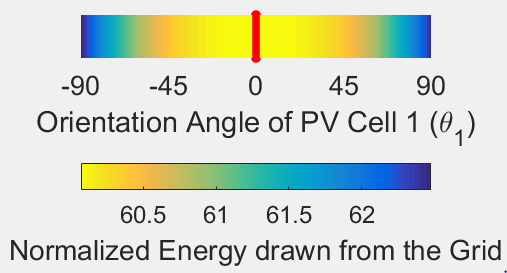
\includegraphics[scale=0.45]{pictures/results/rein_1PV_scale1_offset1_con}  & \vspace{0.1cm} 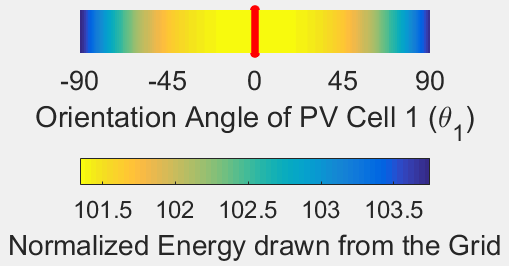
\includegraphics[scale=0.45]{pictures/results/rein_1PV_scale1_offset1_bis}  & \vspace{0.1cm} 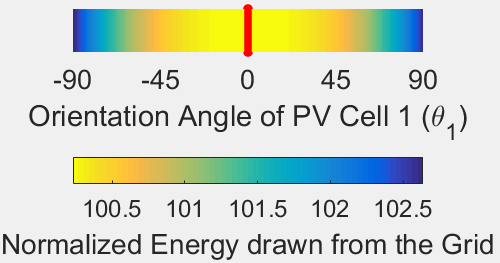
\includegraphics[scale=0.45]{pictures/results/rein_1PV_scale1_offset1_res} \\
			
			 	
							  &  $\quad C(t)= 1$  &   $\quad C(t)=C_{\mathrm{bus}}(t) + 1$ &  $\quad C(t)=C_{\mathrm{res}}(t) + 1$ \\ 	
									
									&  (Figure \ref{constant_allgemein} yellow line)  &   (Figure \ref{business_allgemein} yellow line)&  (Figure \ref{residential_allgemein} yellow line) \\  \hline 		
				   &  Table cell (d): & Table cell (e): &  Table cell (f): \\
						   $G<C$ & \vspace{0.1cm}  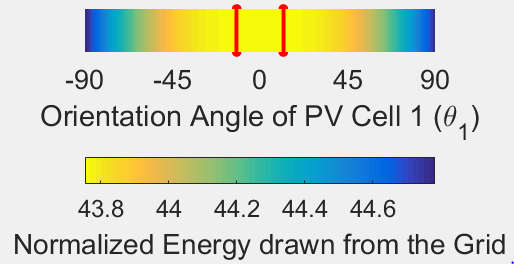
\includegraphics[scale=0.45]{pictures/results/rein_1PV_scale1_offset0_8_con}  & \vspace{0.1cm} 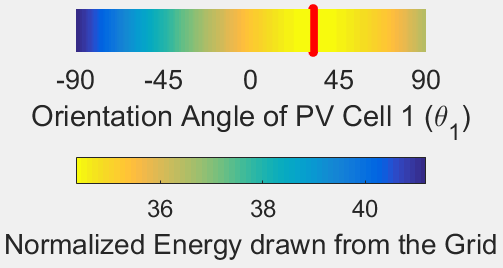
\includegraphics[scale=0.45]{pictures/results/rein_1PV_scale1_offset0_3_bis}  &
      \vspace{0.1cm} 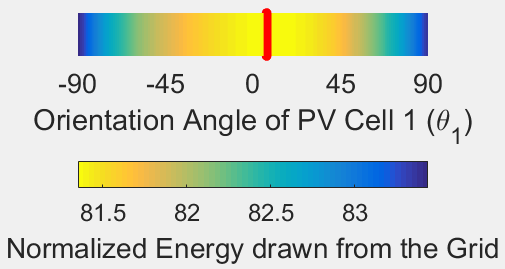
\includegraphics[scale=0.45]{pictures/results/rein_1PV_scale1_offset0_8_res} \\
		
				
					  &   $\quad C(t)= 0.8$  &   $\quad C(t)=C_{\mathrm{bus}}(t) + 0.3$ & $\quad C(t)=C_{\mathrm{res}}(t) + 0.8$\\
						
						  &  (Figure \ref{constant_allgemein} gray line)& (Figure \ref{business_allgemein} green line)&  (Figure \ref{residential_allgemein} green line)\\ \hline
				
				 &  Table cell (g): & Table cell (h): &  Table cell (i): \\
				
				   $G>C$ & \vspace{0.1cm} 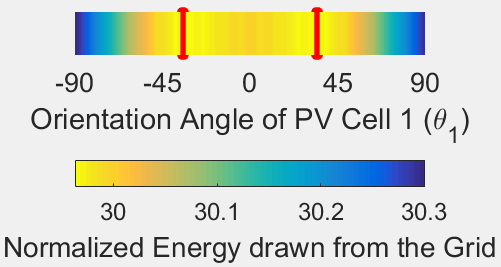
\includegraphics[scale=0.45]{pictures/results/rein_1PV_scale1_offset0_6_con}  & \vspace{0.1cm} 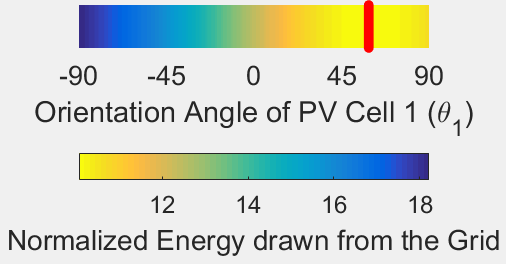
\includegraphics[scale=0.45]{pictures/results/rein_1PV_scale1_offset0_bis}         & \vspace{0.1cm} 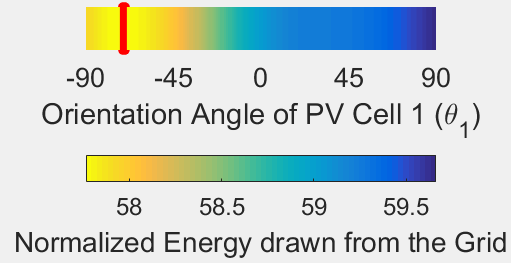
\includegraphics[scale=0.45]{pictures/results/rein_1PV_scale1_offset0_5_res} \\
			
				 &  $\quad C(t)= 0.6$ &   $\quad C(t)=C_{\mathrm{bus}}(t)$ &  $\quad C(t)=C_{\mathrm{res}}(t) + 0.5$ \\  	
				
					 &  (Figure \ref{constant_allgemein} light blue line)&  (Figure \ref{business_allgemein} gray line)&  (Figure \ref{residential_allgemein} gray line)\\  \hline 	
					
						 &  Table cell (j): & Table cell (k): &  Table cell (l): \\
      $G>>C$ &  \vspace{0.1cm} 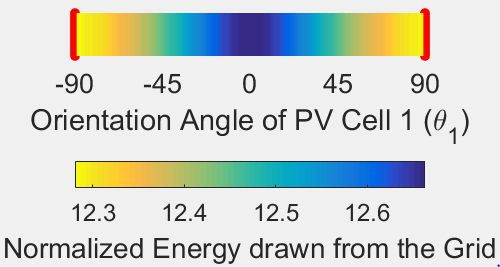
\includegraphics[scale=0.45]{pictures/results/rein_1PV_scale1_offset0_3_con}  & \vspace{0.1cm} 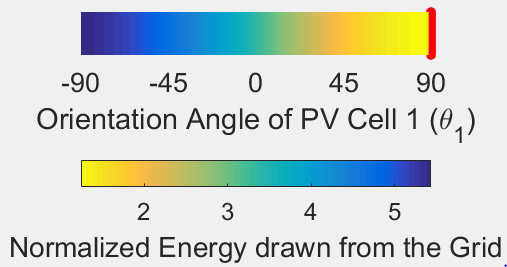
\includegraphics[scale=0.45]{pictures/results/rein_1PV_scale0_5_offset0_bis}  &
      \vspace{0.1cm} 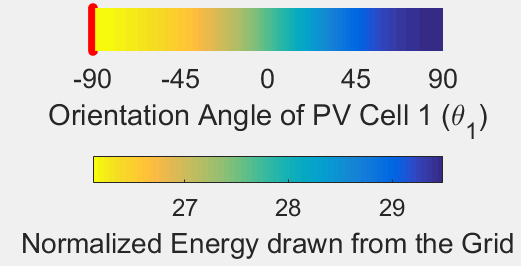
\includegraphics[scale=0.45]{pictures/results/rein_1PV_scale1_offset0_res} \\
			

			&   $\quad C(t)= 0.3$ &   $\quad C(t)=\frac{1}{2}C_{\mathrm{bus}}(t)$ &  $\quad C(t)=C_{\mathrm{res}}(t)$  \\
	
			
			&\vspace{-0.5cm}  (Figure \ref{constant_allgemein} black line)& \vspace{-0.5cm}   (Figure \ref{business_allgemein} light blue line)&\vspace{0.3cm}   (Figure \ref{residential_allgemein} light blue line) 
			
		
  \end{tabular}
\end{table}




\newpage




\subsubsection{Results for 2 PV Cells (N=2) \label{results_2PV}}

Table \ref{table_2PV} and Table \ref{opt_2PV} show the results for 2 PV cells.

The orientation angles are optimized for three different types of load profiles: the constant load profile $C_{\mathrm{con}}(t)$, the business load profile $C_{\mathrm{bus}}(t)$, and the residential load profile $C_{\mathrm{res}}(t)$ (cf. Figure \ref{all_consumption_profiles}). The left, middle, and right columns in Table \ref{table_2PV} represent the constant, business, and residential load profiles, respectively. Each row in Table \ref{table_2PV} represents the relative relationship between the energy generation profile and energy consumption profile. In other words, the first, second, third, and fourth rows in Table \ref{table_2PV} represent the scenario that the energy generation is significantly smaller, is slightly smaller, is slightly greater, is significantly greater than the energy consumption, denoted by $G<<C$, $G<C$, $G>C$, and $G>>C$, respectively. The red points in Table \ref{table_2PV} are the optimal orientation angles.
Each square in Table \ref{table_2PV} has one line of symmetry \mbox{$L$:= \{$(\theta_1,\theta_2)\in [-90^\mathrm{o},90^\mathrm{o}]^2 \enskip|\theta_1=\theta_2$\}}.




\newpage
\settablecounter{2}{5}

\begin{sidewaystable}
 \centering
\captionsetup{justification=centering}
\caption{\\ Summary of all optimal orientation angles for 2 PV cells with the different load profiles from Table \ref{table_2PV} \label{opt_2PV}}
  \begin{tabular}
      {c|c||c|c|c} 
			\multicolumn{2}{c||}{}   &Constant Load Profile  &  Business Load Profile  &  Residential Load Profile  \\
			
      \hline\hline
			
			&&  Table cell (a) of Table \ref{table_2PV}:    &Table cell (b) of Table \ref{table_2PV}:     &Table cell (c) of Table \ref{table_2PV}:     \\  
			  & & 1 optimal point   & 1 optimal point  &1 optimal point   \\  
				
				$G<<C$ &  \  $(\theta_1^*,\theta_2^*)$ \  & $\in \{(0^\mathrm{o},0^\mathrm{o})\}$    & $\in \{(0^\mathrm{o},0^\mathrm{o})\}$ &$\in \{(0^\mathrm{o},0^\mathrm{o})\}$ \\\cline{2-5}		
				
					&   $f(\theta_1^*,\theta_2^*)$ &60.0712  &101.3440 &	100.2310\\\cline{2-5}	
					
					&  $\Delta_2$  &0  & 0 &0\\ \hline
					
					&&  Table cell (d) of Table \ref{table_2PV}:    &Table cell (e) of Table \ref{table_2PV}:     &Table cell (f) of Table \ref{table_2PV}:     \\  
				 & & 2 optimal points     & 1 optimal point   &2 optimal points    \\  
				
			$G<C$ &  \  $(\theta_1^*,\theta_2^*)$ \  &  $\in \{(-48^\mathrm{o},48^\mathrm{o}),(48^\mathrm{o},-48^\mathrm{o})\}$     & $\in \{(32^\mathrm{o},32^\mathrm{o})\}$  &$\in \{(-26^\mathrm{o},35^\mathrm{o}),(35^\mathrm{o},-26^\mathrm{o})\}$  \\\cline{2-5}	
	
	&    $f(\theta_1^*,\theta_2^*)$& 51.0780&  34.3548 & 81.2773\\\cline{2-5}	
		
		&  $\Delta_2$  &0.3918 &  0&	0.0757\\ \hline
				
				
				&&  Table cell (g) of Table \ref{table_2PV}:    &Table cell (h) of Table \ref{table_2PV}:     &Table cell (i) of Table \ref{table_2PV}:     \\  
				 &  &2 optimal points    & 1 optimal point    &2 optimal points    \\  
				
					$G>C$ &  \  $(\theta_1^*,\theta_2^*)$ \  & $\in \{(-69^\mathrm{o},69^\mathrm{o}),(69^\mathrm{o},-69^\mathrm{o})\}$   & $\in \{(59^\mathrm{o},59^\mathrm{o})\}$ & $\in \{(-90^\mathrm{o},90^\mathrm{o}),(90^\mathrm{o},-90^\mathrm{o})\}$ \\\cline{2-5}	
					
							&  $f(\theta_1^*,\theta_2^*)$  &42.7376&   10.0621 &	 57.2246\\\cline{2-5}	
							
							&  $\Delta_2$  &1.0154 &  0&	0.5424\\ \hline
							
							&&  Table cell (j) of Table \ref{table_2PV}:    &Table cell (k) of Table \ref{table_2PV}:     &Table cell (l) of Table \ref{table_2PV}:     \\  
				 & & 2 optimal points    & 1 optimal point    &1 optimal point \\  
				
				$G>>C$ &  \  $(\theta_1^*,\theta_2^*)$ \  & $\in \{(-90^\mathrm{o},90^\mathrm{o}),(90^\mathrm{o},-90^\mathrm{o})\}$  & $\in \{(90^\mathrm{o},90^\mathrm{o})\}$   & 	$\in \{(-90^\mathrm{o},-90^\mathrm{o})\}$\\\cline{2-5}	
				
				&    $f(\theta_1^*,\theta_2^*)$ & 27.8739&  1.2400&26.1165\\\cline{2-5}	
				
				&  $\Delta_2$  & 2.0891&  0&	0\\ 
  \end{tabular}
\end{sidewaystable}


\settablecounter{2}{4}
\begin{table}[H] 
 \centering
\vspace{-0.5cm}\leftskip=-1.5cm
\captionsetup{justification=centering}
\caption{\\ Orientation angles optimization for 2 PV cells with different load profiles \label{table_2PV}}
  \begin{tabular}
      {@{ }m{0.11\columnwidth}@{ }||@{ }M{0.34\columnwidth}@{ }|@{ }M{0.34\columnwidth}@{ }|@{ }M{0.34\columnwidth}@{ }} 
			&  Constant Load Profile &  Business Load Profile & Residential Load Profile \\ \hline\hline
			&  Table cell (a): & Table cell (b): &  Table cell (c): \\
			  $G<<C$ & \vspace{0.1cm}  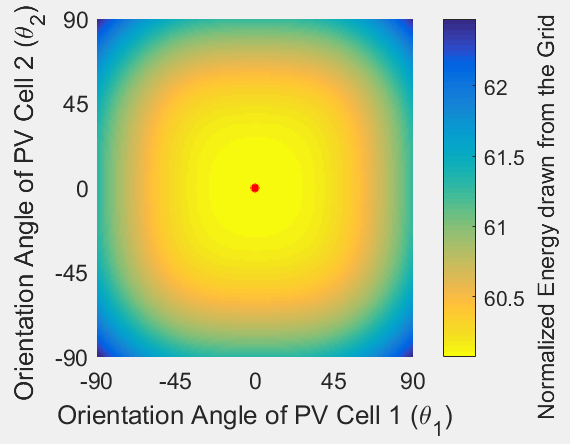
\includegraphics[width=0.34\columnwidth, height=4.5cm]{pictures/results/rein_2PV_scale1_offset1_con}  & \vspace{0.1cm} 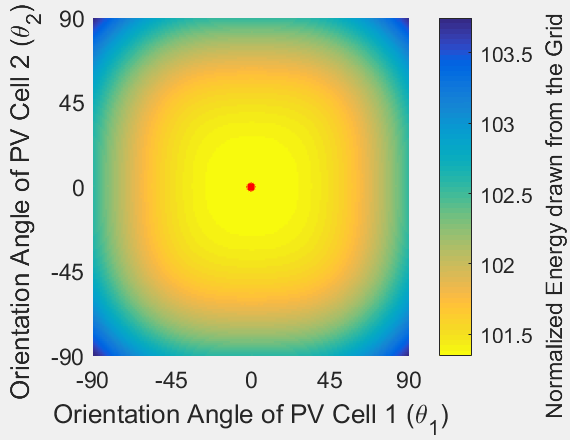
\includegraphics[width=0.34\columnwidth, height=4.5cm]{pictures/results/rein_2PV_scale1_offset1_bis}  &
      \vspace{0.1cm} 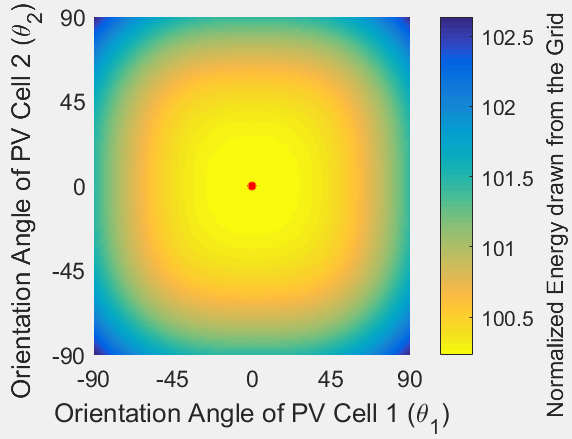
\includegraphics[width=0.34\columnwidth, height=4.5cm]{pictures/results/rein_2PV_scale1_offset1_res} \\
		
			
			
			  &  $\quad C(t)= 1$  &   $\quad C(t)=C_{\mathrm{bus}}(t) + 1$  &  $\quad C(t)=C_{\mathrm{res}}(t) + 1$ \\  		
				
				&  (Figure \ref{constant_allgemein} yellow line)  &  (Figure \ref{business_allgemein} yellow line)&  (Figure \ref{residential_allgemein} yellow line)\\  \hline 		
				&  Table cell (d): & Table cell (e): &  Table cell (f): \\
						   $G<C$ & \vspace{0.1cm}  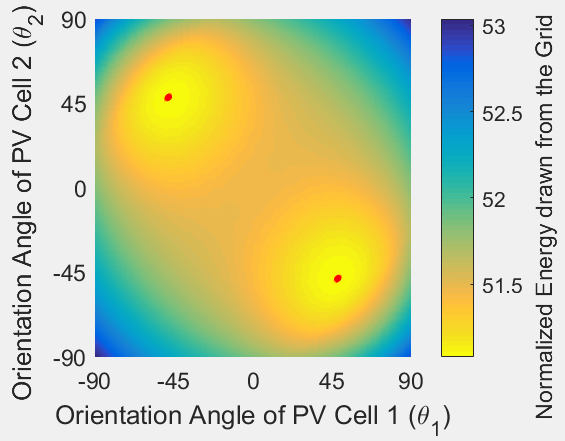
\includegraphics[width=0.34\columnwidth, height=4.5cm]{pictures/results/rein_2PV_scale1_offset0_9_con}  & \vspace{0.1cm} 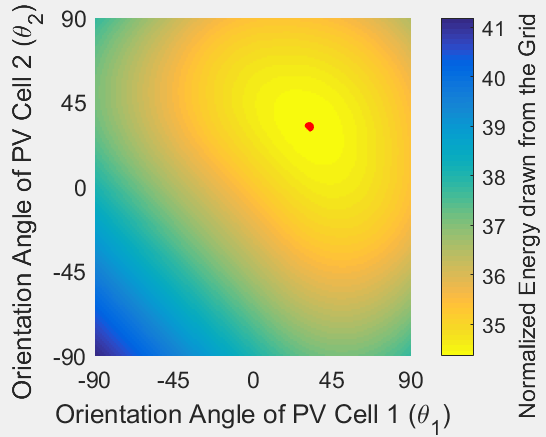
\includegraphics[width=0.34\columnwidth, height=4.5cm]{pictures/results/rein_2PV_scale1_offset0_3_bis}  &
      \vspace{0.1cm} 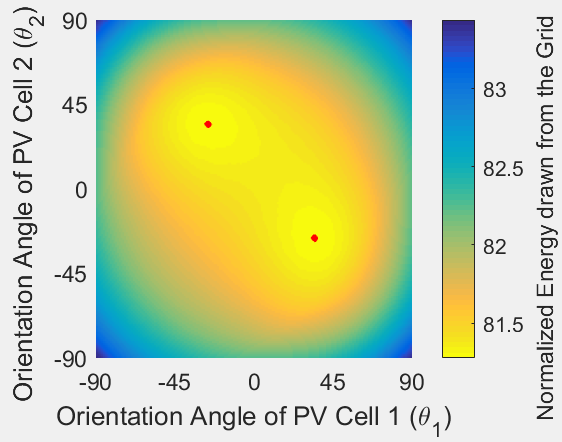
\includegraphics[width=0.34\columnwidth, height=4.5cm]{pictures/results/rein_2PV_scale1_offset0_8_res} \\
			
			  &   $\quad C(t)= 0.9$ &   $\quad C(t)=C_{\mathrm{bus}}(t) + 0.3$ &  $\quad C(t)=C_{\mathrm{res}}(t) + 0.8$ \\  
				
				 &   (Figure \ref{constant_allgemein} green line)&  (Figure \ref{business_allgemein} green line)& (Figure \ref{residential_allgemein} green line)\\ \hline 
				
				&  Table cell (g): & Table cell (h): &  Table cell (i): \\
				  $G>C$ & \vspace{0.1cm} 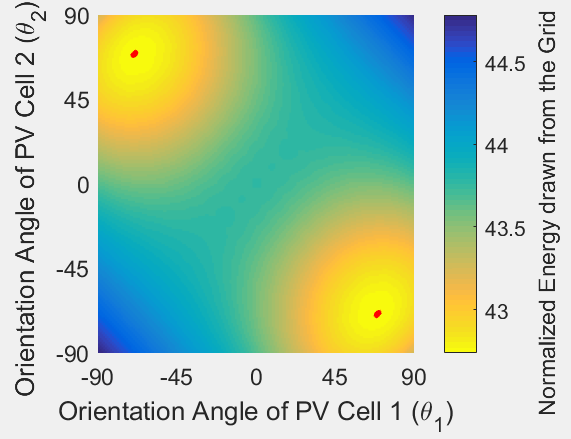
\includegraphics[width=0.34\columnwidth, height=4.5cm]{pictures/results/rein_2PV_scale1_offset0_8_con}  & \vspace{0.1cm} 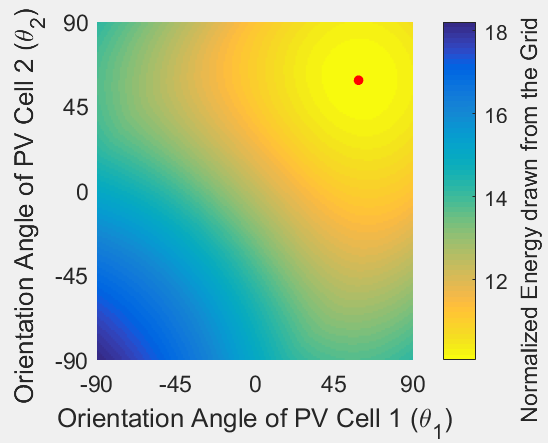
\includegraphics[width=0.34\columnwidth, height=4.5cm]{pictures/results/rein_2PV_scale1_offset0_bis}         & \vspace{0.1cm} 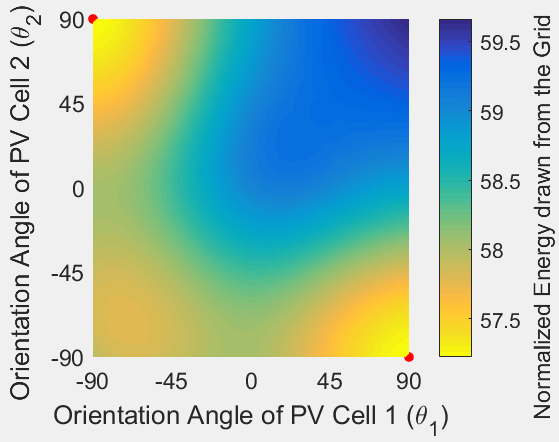
\includegraphics[width=0.34\columnwidth, height=4.5cm]{pictures/results/rein_2PV_scale1_offset0_5_res} \\
			
			  &   $\quad C(t)= 0.8$ &   $\quad C(t)=C_{\mathrm{bus}}(t)$  &  $\quad C(t)=C_{\mathrm{res}}(t) + 0.5$ \\  
					
					&   (Figure \ref{constant_allgemein} gray line)&  (Figure \ref{business_allgemein} gray line)&  (Figure \ref{residential_allgemein} gray line)\\  \hline 	
						
						&  Table cell (j): & Table cell (k): &  Table cell (l): \\
      $G>>C$ &  \vspace{0.1cm} 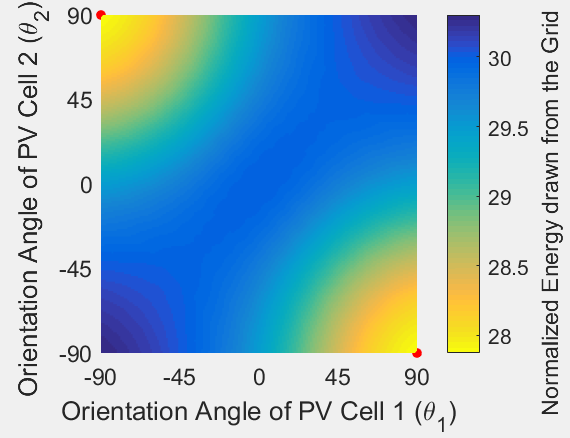
\includegraphics[width=0.34\columnwidth, height=4.5cm]{pictures/results/rein_2PV_scale1_offset0_6_con}  & \vspace{0.1cm} 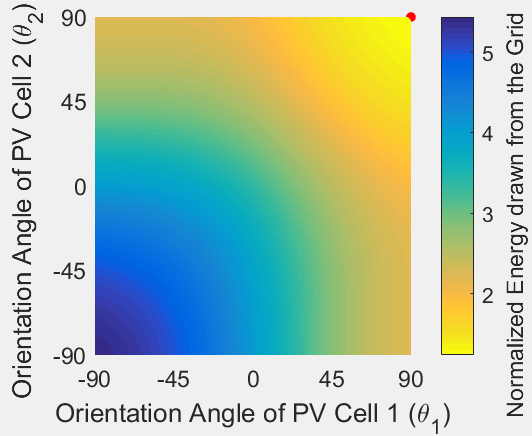
\includegraphics[width=0.34\columnwidth, height=4.5cm]{pictures/results/rein_2PV_scale0_5_offset0_bis}  &
      \vspace{0.1cm} 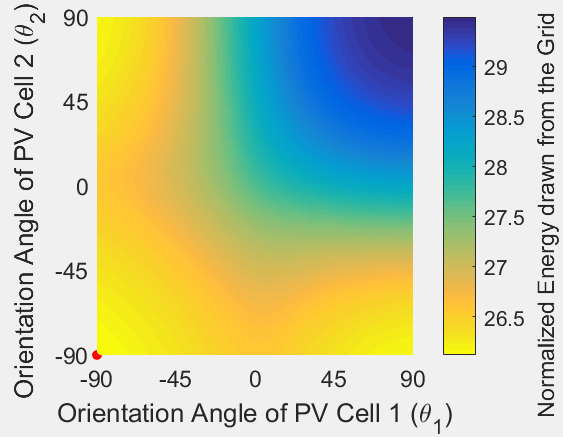
\includegraphics[width=0.34\columnwidth, height=4.5cm]{pictures/results/rein_2PV_scale1_offset0_res} \\
			
			  &   $\quad C(t)= 0.6$ &   $\quad C(t)=\frac{1}{2}C_{\mathrm{bus}}(t)$  & $\quad C(t)=C_{\mathrm{res}}(t) $ \\
				
							  & \vspace{-0.2cm}  (Figure \ref{constant_allgemein} light blue line)&  \vspace{-0.2cm}  (Figure \ref{business_allgemein} light blue line)&\vspace{0.3cm}   (Figure \ref{residential_allgemein} light blue line) 
			
		
  \end{tabular}
\end{table}


\newpage


\subsubsection{Results for 3 PV Cells (N=3) \label{results_3PV}}

Table \ref{table_3PV} and Table \ref{opt_3PV} show the results for 3 PV cells.

The orientation angles are optimized for three different types of load profiles: the constant load profile $C_{\mathrm{con}}(t)$, the business load profile $C_{\mathrm{bus}}(t)$, and the residential load profile $C_{\mathrm{res}}(t)$ (cf. Figure \ref{all_consumption_profiles}). The left, middle, and right columns in Table \ref{table_3PV} represent the constant, business, and residential load profiles, respectively. Each row in Table \ref{table_3PV} represents the relative relationship between the energy generation profile and energy consumption profile. In other words, the first, second, third, and fourth rows in Table \ref{table_3PV} represent the scenario that the energy generation is significantly smaller, is slightly smaller, is slightly greater, is significantly greater than the energy consumption, denoted by $G<<C$, $G<C$, $G>C$, and $G>>C$, respectively. The red points in each cube in Table \ref{table_3PV} are the optimal orientation angles.
Each cube in Table \ref{table_3PV} has three planes of symmetry as follows:


\begin{align}
&P_1:= \{(\theta_1,\theta_2,\theta_3)\in [-90^\mathrm{o},90^\mathrm{o}]^3 \enskip|\theta_2=\theta_3\},\\ 
&P_2:= \{(\theta_1,\theta_2,\theta_3)\in [-90^\mathrm{o},90^\mathrm{o}]^3 \enskip |\theta_1=\theta_3\}, \text{ and}\\ 
&P_3:= \{(\theta_1,\theta_2,\theta_3)\in [-90^\mathrm{o},90^\mathrm{o}]^3 \enskip |\theta_1=\theta_2\}.
\end{align}

The y-axis ($\theta_2$-axis) is reversed in all business load profile scenarios (second column of Table \ref{table_3PV}) so that the optimal points (red points) are visible. Because it is not possible to show all values from a solid 3D cube on a 2D paper, every solid cube in Table \ref{table_3PV} is visualized by 6 planes slicing through the cube. The six planes are

\begin{align}
&S_1:= \{(\theta_1,\theta_2,\theta_3)\in [-90^\mathrm{o},90^\mathrm{o}]^3 \enskip|\theta_3=90^\mathrm{o}\}, \\
&S_2:= \{(\theta_1,\theta_2,\theta_3)\in [-90^\mathrm{o},90^\mathrm{o}]^3 \enskip|\theta_3=45^\mathrm{o}\}, \\
&S_3:= \{(\theta_1,\theta_2,\theta_3)\in [-90^\mathrm{o},90^\mathrm{o}]^3 \enskip|\theta_3=0^\mathrm{o}\}, \\
&S_4:= \{(\theta_1,\theta_2,\theta_3)\in [-90^\mathrm{o},90^\mathrm{o}]^3 \enskip|\theta_3=-45^\mathrm{o}\},\\ 
&S_5:= \{(\theta_1,\theta_2,\theta_3)\in [-90^\mathrm{o},90^\mathrm{o}]^3 \enskip|\theta_3=-90^\mathrm{o}\}, \text{ and}\\ 
&S_6:= \{(\theta_1,\theta_2,\theta_3)\in [-90^\mathrm{o},90^\mathrm{o}]^3 \enskip|\theta_2=0^\mathrm{o}\}.
\end{align}

The optimal orientation angles (red points in Table \ref{table_3PV}) might float between the six slicing planes. Table \ref{opt_3PV} presents the exact values of the optimal orientation angles, hence the exact position of the red points in the cube. 



\newpage



\settablecounter{2}{7}
\begin{sidewaystable}
\centering
\captionsetup{justification=centering}
\caption{\\ Summary of all optimal orientation angles for 3 PV cells with the different load profiles from Table \ref{table_3PV} \label{opt_3PV}}
  \begin{tabular}
      {c|c||c|c|c} 
			\multicolumn{2}{c||}{ }& Constant Load Profile & Business Load Profile   &  Residential Load Profile  \\
			
      \hline\hline
			
			&&  Table cell (a) of Table \ref{table_3PV}:    &Table cell (b) of Table \ref{table_3PV}:     &Table cell (c) of Table \ref{table_3PV}:     \\  
			  &  &  1 optimal point     & 1 optimal point   &1 optimal point    \\  
				
				$G<<C$ &     $(\theta_1^*,\theta_2^*,\theta_3^*)$      &   $\in \{(0^\mathrm{o},0^\mathrm{o},0^\mathrm{o})\}$      &     $\in \{(0^\mathrm{o},0^\mathrm{o},0^\mathrm{o})\}$&         $\in \{(0^\mathrm{o},0^\mathrm{o},0^\mathrm{o})\}$   \\\cline{2-5}		
				
				&  $f(\theta_1^*,\theta_2^*,\theta_3^*)$  &60.0712& 101.3440&	 100.2310\\\cline{2-5}	
				
				&  $\Delta_3$  &0  &0 &	0\\ \hline
				
				
							&&  Table cell (d) of Table \ref{table_3PV}:    &Table cell (e) of Table \ref{table_3PV}:     &Table cell (f) of Table \ref{table_3PV}:     \\  
	  &&  6 optimal points    &1 optimal point    &3 optimal points   \\ 
				
		
				
		 &	$(\theta_1^*,\theta_2^*,\theta_3^*)$ 	&    $\in \{(-55^\mathrm{o},42^\mathrm{o},42^\mathrm{o})$, $(-42^\mathrm{o},-42^\mathrm{o},55^\mathrm{o})$,   & & 	$\in \{(-33^\mathrm{o},31^\mathrm{o},31^\mathrm{o})$,  \\ 
			 	
	$G<C$ 		 &&     $(-42^\mathrm{o},55^\mathrm{o},-42^\mathrm{o})$, $(42^\mathrm{o},-55^\mathrm{o},42^\mathrm{o})$, &$\in \{(32^\mathrm{o},32^\mathrm{o},32^\mathrm{o})\}$&  $(31^\mathrm{o},-33^\mathrm{o},31^\mathrm{o})$,  \\ 
				
			 &	& $(42^\mathrm{o},42^\mathrm{o},-55^\mathrm{o})$, $(55^\mathrm{o},-42^\mathrm{o},-42^\mathrm{o})\}$& &   $(31^\mathrm{o},31^\mathrm{o},-33^\mathrm{o})\}$ \\\cline{2-5}	
			
			&    $f(\theta_1^*,\theta_2^*,\theta_3^*)$        &     51.1204     &34.3548&   81.2783  \\\cline{2-5}	
				
							&  $\Delta_3$  &-0.0424 &  0 &	-0.001\\ \hline	
				
				
							&&  Table cell (g) of Table \ref{table_3PV}:    &Table cell (h) of Table \ref{table_3PV}:     &Table cell (i) of Table \ref{table_3PV}:     \\  
				&    &  6 optimal points    &1 optimal point    &3 optimal points  \\ 
				
				
				&$(\theta_1^*,\theta_2^*,\theta_3^*)$  & $\in \{(-76^\mathrm{o},60^\mathrm{o},60^\mathrm{o})$, $(-60^\mathrm{o},-60^\mathrm{o},76^\mathrm{o})$,  & &	$\in \{(-85^\mathrm{o},-85^\mathrm{o},87^\mathrm{o})$, \\ 
				
				$G>C$ 	& &  $(-60^\mathrm{o},76^\mathrm{o},-60^\mathrm{o})$, $(60^\mathrm{o},-76^\mathrm{o},60^\mathrm{o})$,&  $\in \{(59^\mathrm{o},59^\mathrm{o},59^\mathrm{o})\}$ &	$(-85^\mathrm{o},87^\mathrm{o},-85^\mathrm{o})$, \\ 
				
					& & $(60^\mathrm{o},60^\mathrm{o},-76^\mathrm{o})$, $(76^\mathrm{o},-60^\mathrm{o},-60^\mathrm{o})\}$  & &	 $(87^\mathrm{o},-85^\mathrm{o},-85^\mathrm{o})\}$ \\\cline{2-5}	
					
								&       $f(\theta_1^*,\theta_2^*,\theta_3^*)$    &      42.8827   & 10.0621      &   57.2542    \\\cline{2-5}		
					
					&  $\Delta_3$  &-0.1451 &  0&	-0.0296\\ \hline		
				
				
							&&  Table cell (j) of Table \ref{table_3PV}:    &Table cell (k) of Table \ref{table_3PV}:     &Table cell (l) of Table \ref{table_3PV}:     \\  
				&  & 6 optimal points    & 1 optimal point   &3 optimal points    \\ 
				
				
				& $(\theta_1^*,\theta_2^*,\theta_3^*)$ &    $\in \{(-90^\mathrm{o},-90^\mathrm{o},90^\mathrm{o})$, $(-90^\mathrm{o},90^\mathrm{o},-90^\mathrm{o})$, & &	$\in \{(-90^\mathrm{o},-90^\mathrm{o},90^\mathrm{o})$,\\
					$G>>C$ 	&&    $(-90^\mathrm{o},90^\mathrm{o},90^\mathrm{o})$, $(90^\mathrm{o},-90^\mathrm{o},-90^\mathrm{o})$,  &  $\in \{(90^\mathrm{o},90^\mathrm{o},90^\mathrm{o})\}$&	 $(-90^\mathrm{o},90^\mathrm{o},-90^\mathrm{o})$,\\			

				&&    $(90^\mathrm{o},-90^\mathrm{o},90^\mathrm{o})$, $(90^\mathrm{o},90^\mathrm{o},-90^\mathrm{o})\}$ & &	 $(90^\mathrm{o},-90^\mathrm{o},-90^\mathrm{o})\}$\\\cline{2-5}
					
							&      $f(\theta_1^*,\theta_2^*,\theta_3^*)$    &     28.2100   &     1.2400   &   25.9671    \\\cline{2-5}		
				
				&  $\Delta_3$  & -0.3361& 0 &	0.1494
  \end{tabular}
\end{sidewaystable}




\settablecounter{2}{6}
\begin{table}[H] 
 \centering
\vspace{-0.5cm}\leftskip=-1.5cm
\captionsetup{justification=centering}
\caption{\\ Orientation angles optimization for 3 PV cells with different load profiles \label{table_3PV} }
  \begin{tabular}
      {@{ }m{0.11\columnwidth}@{ }||@{ }M{0.34\columnwidth}@{ }|@{ }M{0.34\columnwidth}@{ }|@{ }M{0.34\columnwidth}@{ }} 
			&  Constant Load Profile &  Business Load Profile & Residential Load Profile \\
			
      \hline\hline 
			
			&  Table cell (a): & Table cell (b): &  Table cell (c): \\
			$G<<C$ &  \vspace{0.1cm}  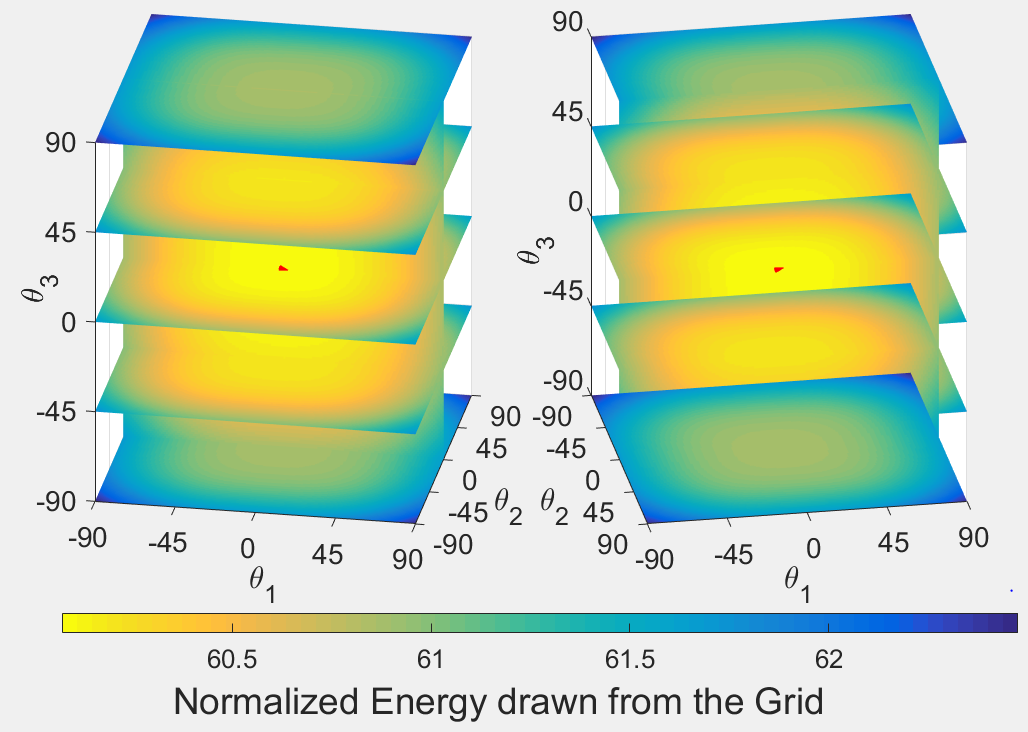
\includegraphics[width=0.34\columnwidth, height=4.6cm]{pictures/results/rein_3PV_scale1_offset1_con}  & \vspace{0.1cm} 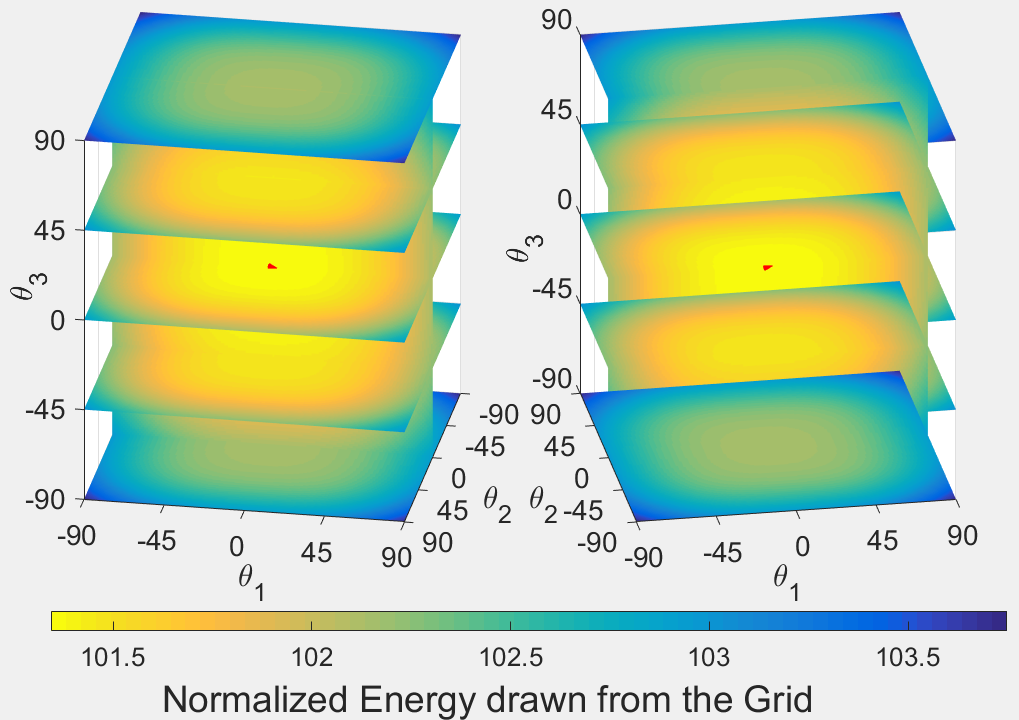
\includegraphics[width=0.34\columnwidth, height=4.6cm]{pictures/results/rein_3PV_scale1_offset1_bis}  & \vspace{0.1cm} 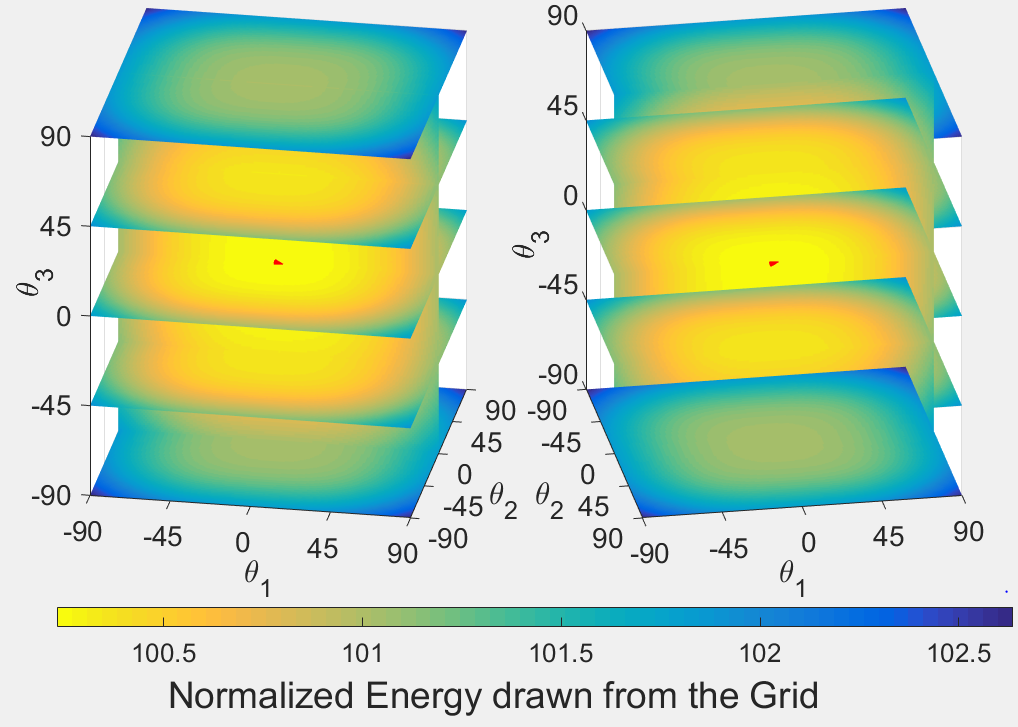
\includegraphics[width=0.34\columnwidth, height=4.6cm]{pictures/results/rein_3PV_scale1_offset1_res} \\
			

						  &   $\quad C(t)= 1$  &   $\quad C(t)=C_{\mathrm{bus}}(t) + 1$ &  $\quad C(t)=C_{\mathrm{res}}(t) + 1$\\  		
							
							 &   (Figure \ref{constant_allgemein} yellow line)  &  (Figure \ref{business_allgemein} yellow line)& (Figure \ref{residential_allgemein} yellow line)\\  \hline 		
				&  Table cell (d): & Table cell (e): &  Table cell (f): \\
						   $G<C$ & \vspace{0.1cm}  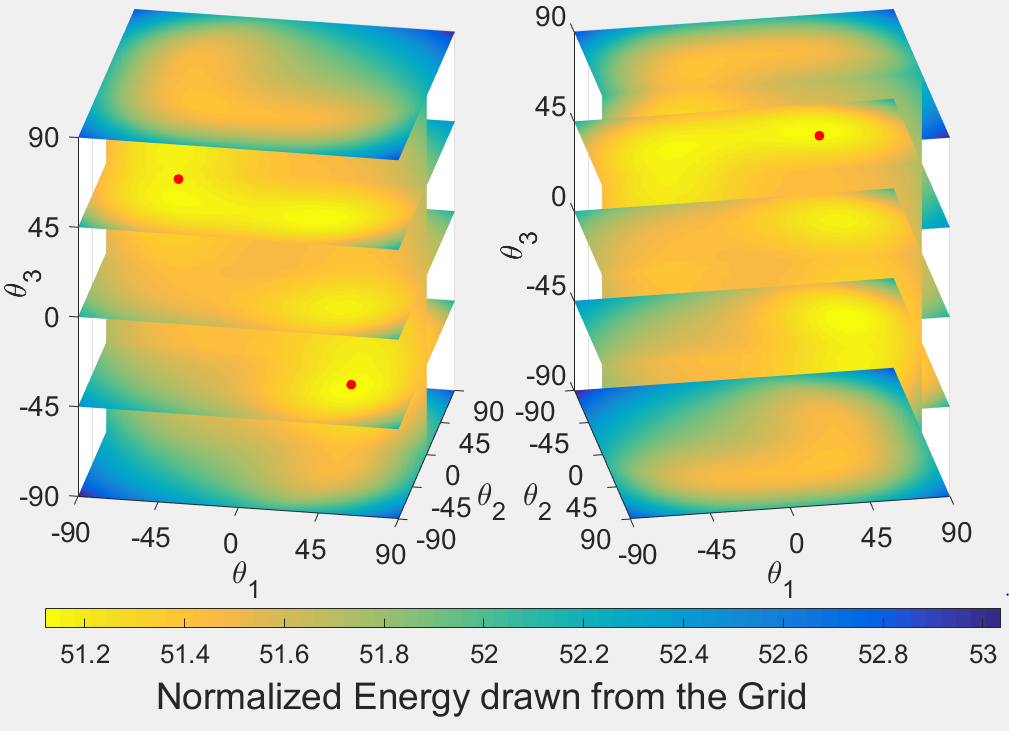
\includegraphics[width=0.34\columnwidth, height=4.6cm]{pictures/results/rein_3PV_scale1_offset0_9_con}  & \vspace{0.1cm} 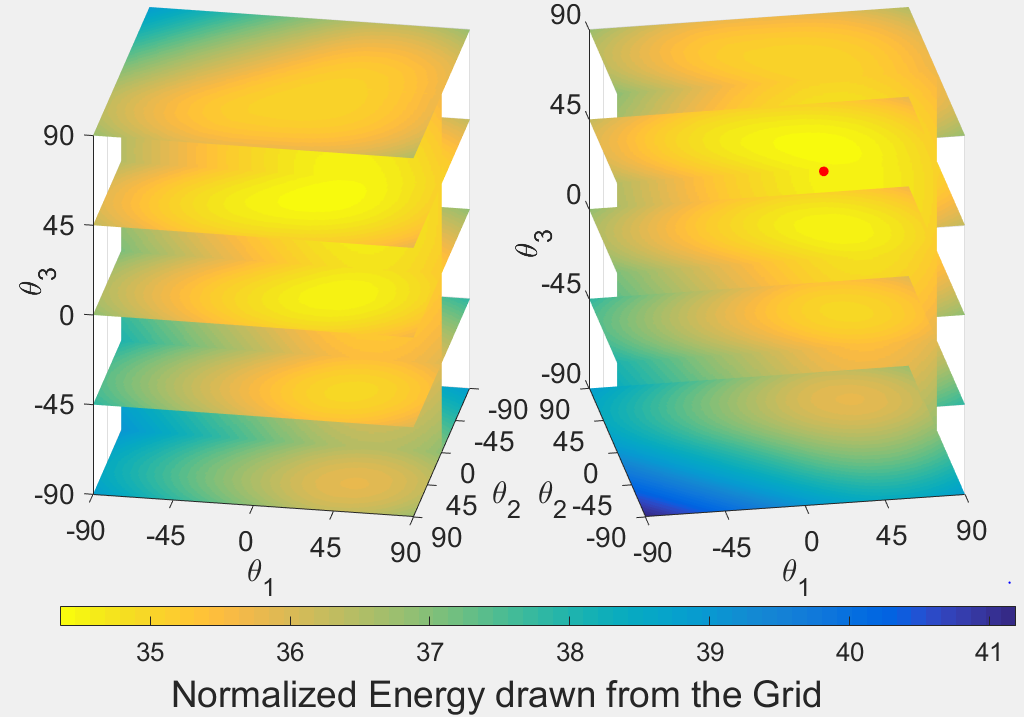
\includegraphics[width=0.34\columnwidth, height=4.6cm]{pictures/results/rein_3PV_scale1_offset0_3_bis}  &
      \vspace{0.1cm} 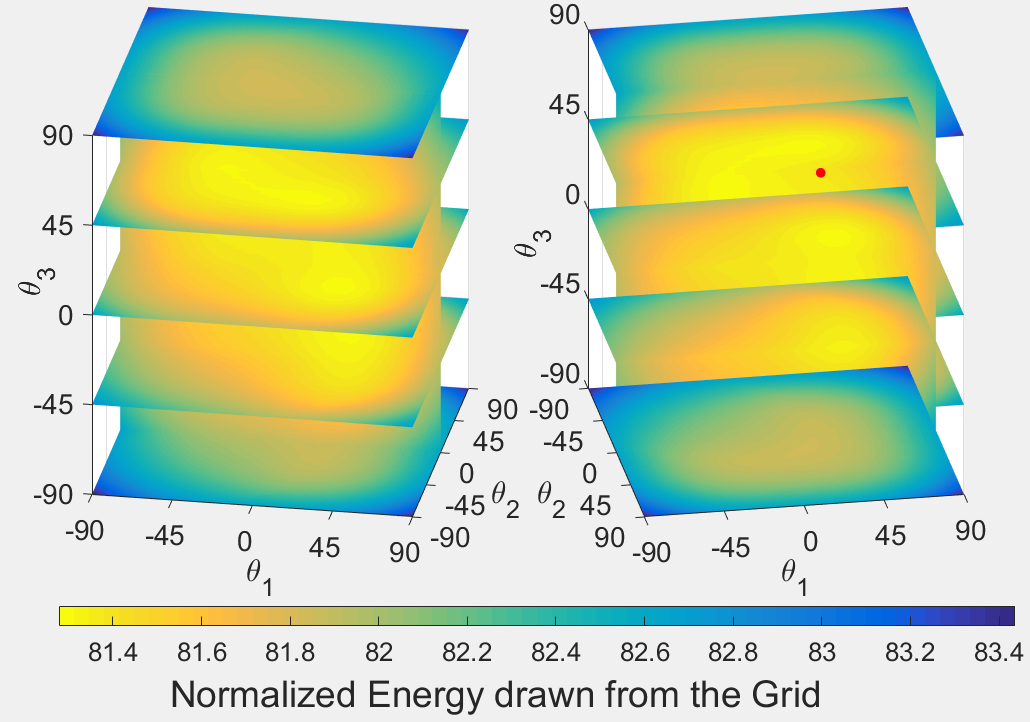
\includegraphics[width=0.34\columnwidth, height=4.6cm]{pictures/results/rein_3PV_scale1_offset0_8_res} \\
		
			&   $\quad C(t)= 0.9$  &  $\quad C(t)=C_{\mathrm{bus}}(t) + 0.3$ &  $\quad C(t)=C_{\mathrm{res}}(t) + 0.8$ \\ 
			
						  &   (Figure \ref{constant_allgemein} green line)&  (Figure \ref{business_allgemein} green line)&  (Figure \ref{residential_allgemein} green line)\\ \hline  
				
				&  Table cell (g): & Table cell (h): &  Table cell (i): \\
				  $G>C$ & \vspace{0.1cm} 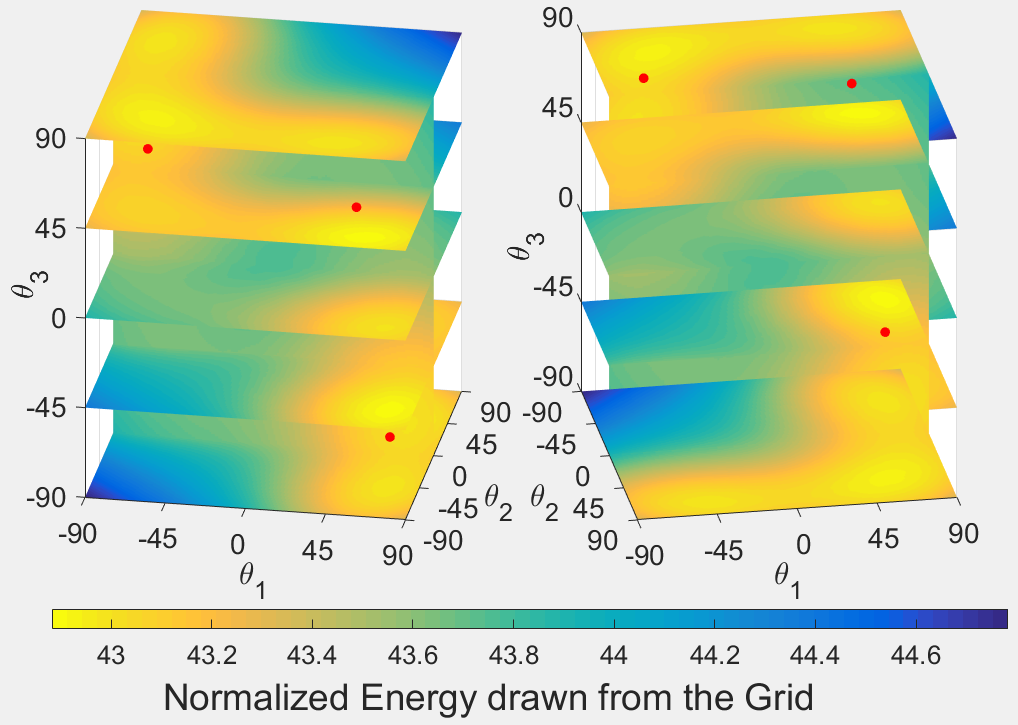
\includegraphics[width=0.34\columnwidth, height=4.6cm]{pictures/results/rein_3PV_scale1_offset0_8_con}  & \vspace{0.1cm} 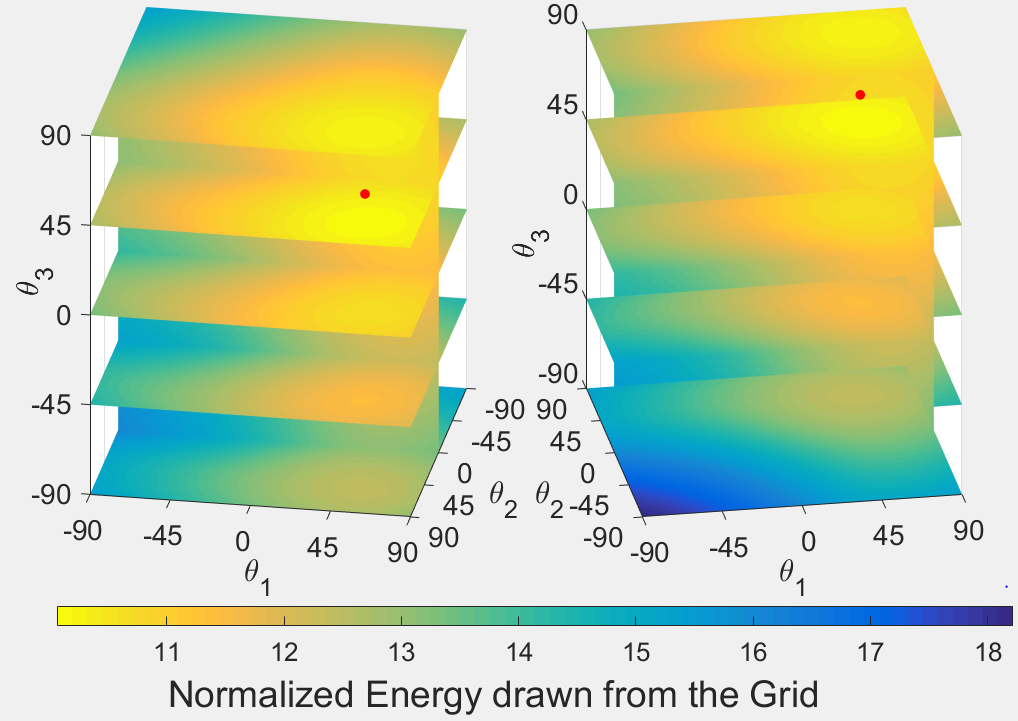
\includegraphics[width=0.34\columnwidth, height=4.6cm]{pictures/results/rein_3PV_scale1_offset0_bis}         & \vspace{0.1cm} 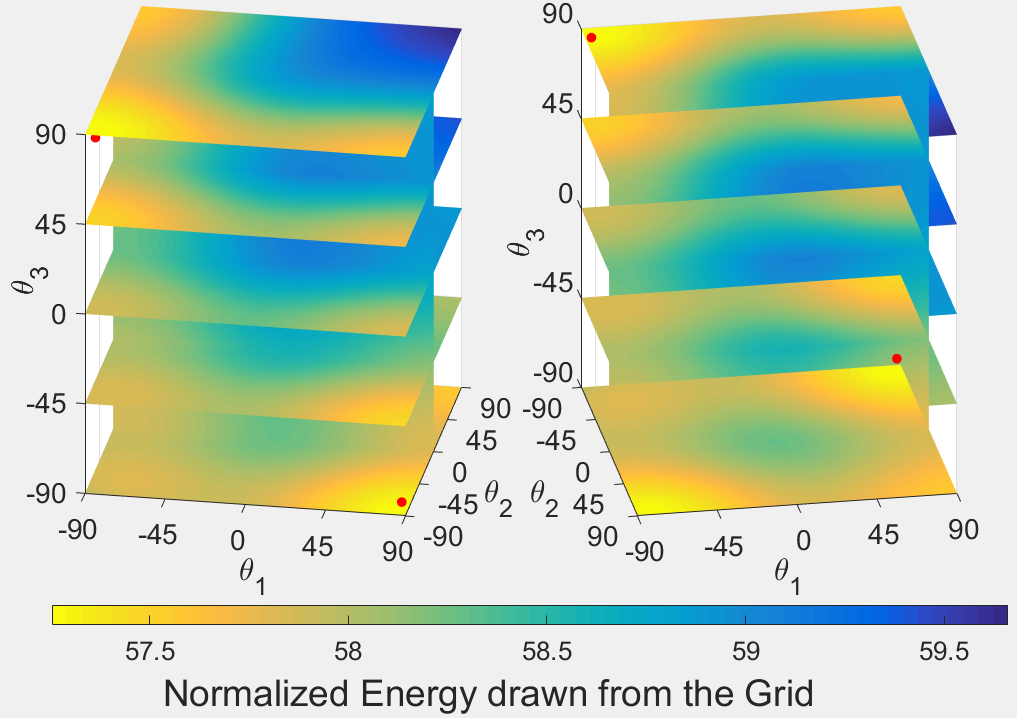
\includegraphics[width=0.34\columnwidth, height=4.6cm]{pictures/results/rein_3PV_scale1_offset0_5_res}\\
			
			&   $\quad C(t)= 0.8$ &   $\quad C(t)=C_{\mathrm{bus}}(t)$  &  $\quad C(t)=C_{\mathrm{res}}(t) + 0.5$ \\  
			
					  &  (Figure \ref{constant_allgemein} gray line)&   (Figure \ref{business_allgemein} gray line)& (Figure \ref{residential_allgemein} gray line)\\  \hline 	
						
						
						&  Table cell (j): & Table cell (k): &  Table cell (l): \\
      $G>>C$ &  \vspace{0.1cm} 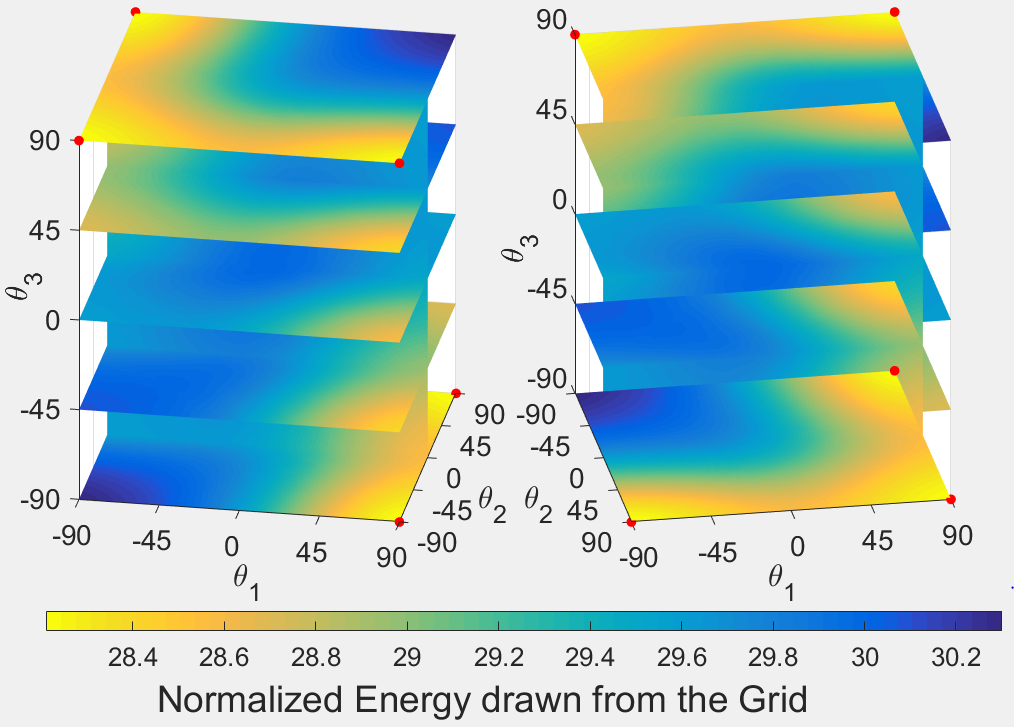
\includegraphics[width=0.34\columnwidth, height=4.6cm]{pictures/results/rein_3PV_scale1_offset0_6_con}  & \vspace{0.1cm} 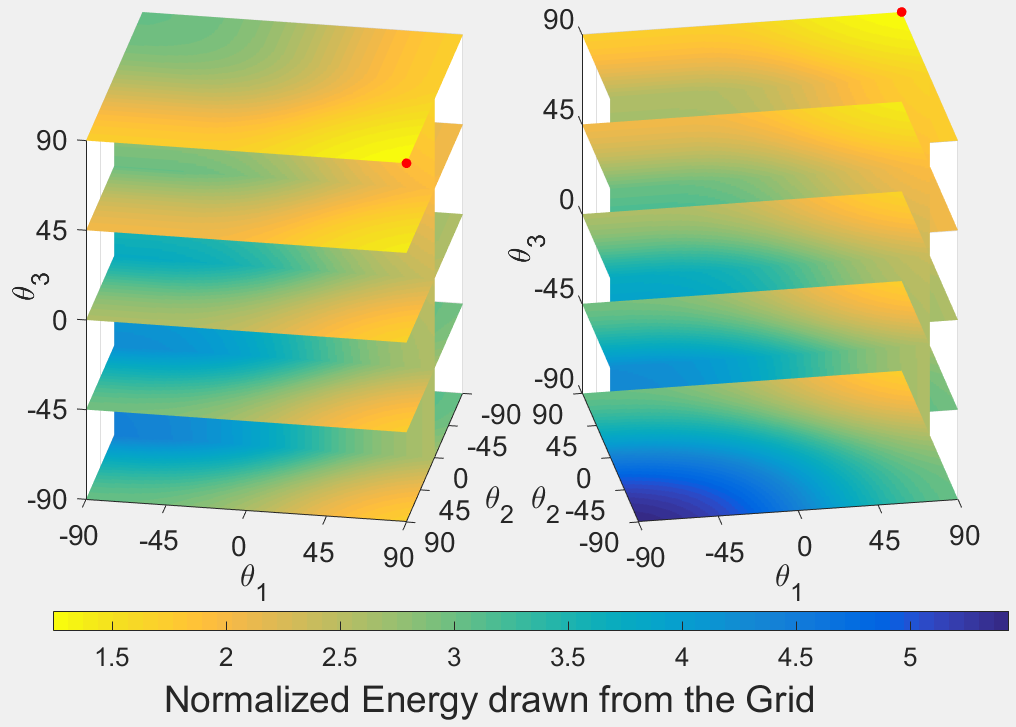
\includegraphics[width=0.34\columnwidth, height=4.6cm]{pictures/results/rein_3PV_scale0_5_offset0_bis}  &
      \vspace{0.1cm} 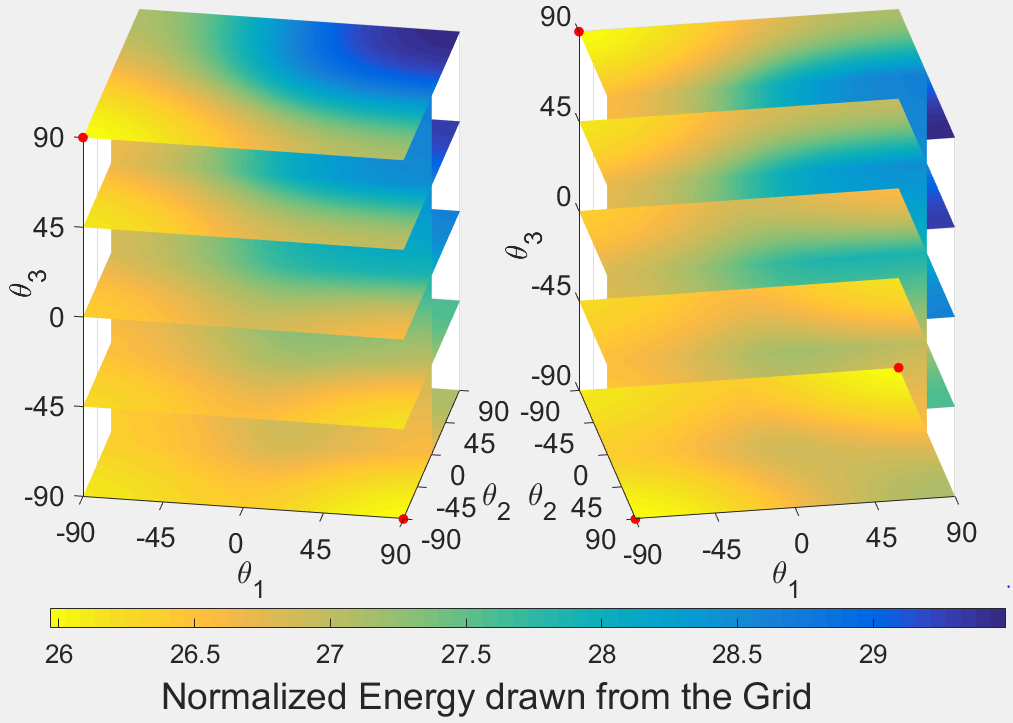
\includegraphics[width=0.34\columnwidth, height=4.6cm]{pictures/results/rein_3PV_scale1_offset0_res} \\
			
			
				  &   $\quad C(t)= 0.6$&   $\quad C(t)=\frac{1}{2}C_{\mathrm{bus}}(t)$  &  $\quad C(t)=C_{\mathrm{res}}(t) $ \\ 
			
			&\vspace{-0.2cm} (Figure \ref{constant_allgemein} light blue line)& \vspace{-0.2cm}  (Figure \ref{business_allgemein} light blue line)& \vspace{0.3cm}  (Figure \ref{residential_allgemein} light blue line)
		
  \end{tabular}
\end{table}







\newpage



\subsection{Summary of the Key Findings and Discussions of the Results\label{findings}}

To evaluate the effects of different numbers of PV cells, the same consumption profile $C(t)$ is used among corresponding table cells in different tables whenever possible.  For example, the table cell (a) of Table \ref{table_1PV} corresponds to the table cell (a) of Table \ref{table_2PV} and to the table cell (a) of Table \ref{table_3PV}. The comparisons between the different tables are fair because the total surface area $A$ is constant. In other words, there will be no more surface area added by adding another PV cell, instead the total surface area $A$ is divided among $N$ PV cells in each scenario. The only exception is that the table cells (d), (g), and (j) of Table \ref{table_1PV} cannot be compared directly to Table \ref{table_2PV} or Table \ref{table_3PV} because their energy consumption profile $C(t)$ is different. 

From a practical point of view, the optimization algorithm is faster for only a few PV cells (1 or 2 PV cells) than for several PV cells (more than 2 PV cells). In addition, if there are several PV cells with different optimal orientation angles, the spacing between the differently oriented PV cells has to be sufficient enough to avoid shadowing effects on the panels. This increases the area needed for deployment of the PV cells. Furthermore, it is not possible to mount PV cells with different orientation angles on the same array or support structure which increases the material cost for buying several arrays or support structures. Hence, it is recommended to use as less differently oriented PV cells as possible.


If $G << C$ (first rows in Table \ref{opt_1PV}, Table \ref{opt_2PV}, and Table \ref{opt_3PV}), all PV cells should be oriented towards the south, i.e., the optimal orientation angles are $\theta_1^*=\theta_2^*=...=\theta_N^*=0^\mathrm{o}$. If $G << C$, the optimal orientation angles are independent of the shape of the energy consumption profile.

The optimal orientation angles change from south orientation in the $G << C$ scenarios towards the east and/or west orientation in the $G >> C$ scenarios in every column of the Table \ref{table_1PV}, Table \ref{table_2PV}, and Table \ref{table_3PV}. The optimal orientation angles in the $G < C$ scenarios are closer to the south orientation than the east and/or west orientation, whereas the optimal orientation angles in the $G > C$ scenarios are closer to the east and/or west orientation than the south orientation.

The gains of adding the first, second, and third PV cell with optimized orientation angle to the system model 1 are evaluated in the following paragraphs.
\subsubsection{PV Cells with Default Orientation Angles}
The centers of the stripes, squares, and cubes in Table \ref{table_1PV}, Table \ref{table_2PV}, and Table \ref{table_3PV} are the normalized energy drawn
from the main grid, i.e, $f(0^\mathrm{o})$, $f(0^\mathrm{o},0^\mathrm{o})$, and $f(0^\mathrm{o},0^\mathrm{o},0^\mathrm{o})$, if no orientation angle optimization is performed, respectively. PV cells are oriented towards the south in the northern hemisphere by default (cf. Table \ref{over}). $f(0^\mathrm{o})=f(0^\mathrm{o},0^\mathrm{o})=f(0^\mathrm{o},...,0^\mathrm{o})$ if the same consumption profile $C(t)$ is used because the total surface area $A$ in the system model 1 is constant. For example, $f(0^\mathrm{o})$ in Table \ref{table_1PV}(a) equals to $f(0^\mathrm{o},0^\mathrm{o})$ in Table \ref{table_2PV}(a) and $f(0^\mathrm{o},0^\mathrm{o},0^\mathrm{o})$ in Table \ref{table_3PV}(a). 

\subsubsection{Adding the First PV Cell with Optimized Orientation Angle}
A positive (negative) $\Delta_1$ value represents an improvement (deterioration) in performance of the system if the first PV cell is added. 
$\Delta_1>0$ for the table cells (d)-(l) and $\Delta_1=0$ for the table cells (a)-(c) in Table \ref{opt_1PV}. The greatest $\Delta_1$ values for the constant, business, and residential load profiles in Table \ref{opt_1PV} are $0.3829$ (table cell (j)), $2.3318$ (table cell (h)), and $1.5493$ (table cell (l)), respectively. The optimized values $f(\theta_1^*)$ (red lines in Table \ref{table_1PV}) are usually significantly greater than the default values $f(0^\mathrm{o})$ (centers of the stripes in Table \ref{table_1PV}). In other words, orientation angle optimization improves the system performance in most scenarios. $\Delta_1$ is always greater or equal to $0$ because $f(0^\mathrm{o})\geq f(\theta_1^*)$. That means the system performance can only be improved and will never worsen by adding the first PV cell. It should be pointed out that a load profile type can have an optimal orientation angle on the east side ($\theta^*<0^{\mathrm{o}}$), on the west side ($\theta^*>0^{\mathrm{o}}$), as well as oriented southwards ($\theta^*=0^{\mathrm{o}}$) in different scenarios as it can be seen for the residential load profiles (third column) in Table \ref{table_1PV}.

\subsubsection{Adding the Second PV Cell with Optimized Orientation Angle} 
$\Delta_2>0$ for all table cells in Table \ref{opt_2PV} with two optimal points, i.e., (d), (f)-(g), and (i)-(j). $\Delta_2=0$ for all table cells in Table \ref{opt_2PV} with only one optimal point, i.e., (a)-(c), (e), (h), and (k)-(l). The greatest $\Delta_2$ values for the constant, business, and residential load profiles in Table \ref{opt_2PV} are $2.0891$ (table cell (j)), $0$ (table cells (b), (e), (h), and (k)), and $0.5424$ (table cell (i)), respectively. The $\Delta_2$ values are usually smaller than the $\Delta_1$ values for the business and residential load profiles, whereas the $\Delta_2$ values are usually greater than the $\Delta_1$ values for the constant load profiles. Consumption profiles which are similar to the constant profile, e.g., the scenarios in the first column, can often improve their performance (\mbox{$\Delta_2>0$}) by choosing orientation angles with opposite algebraic signs, e.g., $\theta_1^*>0^\mathrm{o}$ and \mbox{$\theta_2^*<0^\mathrm{o}$}, as seen in table cells (d), (g), and (j) in Table \ref{opt_2PV}. Consumption profiles which have significant local maxima in the morning as well as in the afternoon, e.g., the residential load profile scenarios in the third column, can often improve their performance ($\Delta_2>0$) by choosing orientation angles with opposite algebraic signs, e.g., $\theta_1^*>0^\mathrm{o}$ and \mbox{$\theta_2^*<0^\mathrm{o}$}, as seen in table cells (f), and (i) in Table \ref{opt_2PV}. Consumption profiles which have only one significant maximum, e.g., the business load profile scenarios in the second column, cannot improve their performance ($\Delta_2=0$) by adding a second PV cell.

\subsubsection{Adding the Third PV Cell with Optimized Orientation Angle} 
$\Delta_3>0$ for the table cell (l) in Table \ref{opt_3PV}. $\Delta_3=0$ for all table cells in Table \ref{opt_3PV} with only one optimal point, i.e., (a)-(c), (e), (h), and (k). $\Delta_3<0$ for the table cells (d), (f)-(g), and (i)-(j) in Table \ref{opt_3PV}. The greatest and lowest $\Delta_3$ values for the constant, business, and residential load profiles in Table \ref{opt_3PV} are $0$ and $-0.3361$, $0$ and $0$, and $0.1494$ and  $-0.0296$, respectively.
The $\Delta_3$ values are usually smaller than the $\Delta_2$ values and sometimes even negative. That means that adding the third PV cell only improves the system performance slightly in some rare scenarios, whereas the system performance worsens in most other scenarios. 
Consumption profiles which are similar to the constant profile worsen their performance ($\Delta_3<0$) in most scenarios because 3 PV cells cannot equally shift the energy generation peak towards the morning and afternoon hours. Either two PV cells have positive algebraic signs and one PV cell has a negative algebraic sign or the other way around, as seen in table cells (d), (g), and (j) in Table \ref{opt_3PV}. 
Consumption profiles which have two significant local maxima in the morning as well as in the afternoon, e.g., the residential load profile scenarios in the third column, can slightly improve ($\Delta_3>0$) or slightly worsen ($\Delta_3<0$) their performance, as seen in table cells (l), and (i) in Table \ref{opt_3PV}.
Consumption profiles which have only one significant maximum, e.g., the business load profile scenarios in the second column, cannot improve their performance (\mbox{$\Delta_3=0$}) by adding a third PV cell.
In general, consumption profiles which have three significant local maxima between sunrise and sunset or consumption profiles which have two significant local maxima (with one maxima significantly greater than the other one) might benefit in some scenarios from 3 PV cells. But it becomes more and more difficult to find such specific consumption profiles and scenarios to justify that 3 or more PV cells are necessary to improve the system performance significantly.



\section{Summary of Chapter \ref{Chapter_1}\label{sum_Chapter_1}}
In Chapter \ref{Chapter_1}, the orientation angles of $N$ PV cells powering one BS were jointly optimized to improve the match between the two profiles on a daily timescale. The energy generation profiles of randomly inclined and oriented PV cells were analytically derived by the irradiance values received at a horizontally-mounted PV cell at the same location. The energy drawn per day from the main grid by the BS given its energy consumption profile was used as the performance metric to determine the optimal set of orientation angels.
The main results are that the system performance ($\Delta_1 > 0$) can be increased significantly by deploying one PV cell with optimal orientation angel $\theta_1^*$ (or several PV cells with the same orientation angle $\theta_1^*$) if the energy generation of the PV cell is slightly smaller ($G<C$), is slightly greater ($G>C$), or is significantly greater ($G>>C$) than the energy consumption of the BS. This is caused by the ability to shift the energy generation peak from noon towards the most significant local maximum between sunrise and sunset of the energy consumption profile. 
Furthermore, the system performance ($\Delta_2 > 0$) can be further increased by deploying two PV cells with jointly optimized orientation angles $\theta_1^*$ and $\theta_2^*$ (or several PV cells where half of them are deployed with $\theta_1^*$ and the other half with $\theta_2^*$) if a constant energy consumption profile or a consumption profile with significant local maxima in the morning as well as in the afternoon are given. This is caused by the ability to shift the energy generation peak from noon towards the morning with east-oriented PV cells, while the other west-oriented PV cells shift the energy generation peak towards the afternoon in the northern hemisphere. Because there are only two directions (morning and afternoon) that the energy can be shifted to, the system performance can not be further increased significantly by deploying more than 2 differently oriented PV cells. More than 2 differently oriented PV cells may even degrade the system performance ($\Delta_3 < 0$) in some scenarios.


